\documentclass[11pt]{article}
\usepackage{graphicx}
\graphicspath{ {images/} }
\usepackage{url}
\usepackage{comment}
\usepackage{epigraph}
\usepackage{float}
\usepackage{wrapfig}
\usepackage{listings}
\usepackage{multirow}
\usepackage{hyperref}
\usepackage{amsfonts}
\usepackage{amsmath}
\usepackage{array}
\usepackage{etoolbox}
\usepackage{relsize}
\usepackage{yax}
\usepackage{hyperref}
\usepackage{textcomp}
\usepackage[english]{babel} 
\usepackage[nodayofweek]{datetime}

\setparameter Cantrell:
 firstname   = Colin
 lastname    = Cantrell
 title       = {Architect \& Engineer}
 email       = {\href{mailto:colin@nexus.io}{colin@nexus.io}}
 
\setparameter April:
 firstname   = April
 lastname    = Bunje
 title       = {Writer}
 email       = {\href{mailto:gramalkin75@yahoo.com}{gramalkin75@yahoo.com}}
 
\setparameter Hauk:
 firstname   = {Nathan}
 lastname    = {Hauk}
 title       = {Security Consultant}
 email       = {\href{mailto:n.hauk79@gmail.com}{n.hauk79@gmail.com}}
 
\setparameter Shea:
 firstname   = {Shea}
 lastname    = {Laver}
 title       = {Writer \& Editor}
 email       = {\href{mailto:danlo@y7mail.com}{danlo@y7mail.com}}
 
\setparameter Victor:
 firstname   = Victor
 lastname    = Moreno
 title       = {Distinguished Engineer}
 email       = {\href{mailto:victor@magooit.com}{victor@magooit.com}}
 
\setparameter BA:
 firstname   = {Brian}
 lastname    = {Anderson}
 title       = {Security Consultant \& Writer}
 email       = {\href{mailto:ba@nexus.io}{ba@nexus.io}}
 
 
\newcommand{\printcontributor}[1]{
  \begingroup
  \parindent 0pt
  \usevalue #1: firstname
  \space
  \usevalue #1: lastname
  \ifattribute #1: title {\par}{\relax}
  \usevalue #1: title
  \ifattribute #1: email {\space-\space} {\par\relax}
  \usevalue #1: email
  \endgroup
}

\newcommand{\maketitlepage}[3]{
  \begingroup
  \centering
   
  \vspace*{2\baselineskip}
  
  \textbf{Written by:}\par
  \medskip
  Colin Cantrell\par

  \vspace*{2\baselineskip}

  \textbf{Contributions by:}\par\medskip
  \renewcommand\do[1]{%
    {
    \usevalue ##1:firstname \space \usevalue ##1:lastname \par}%
    }
  \docsvlist{#1}
  
  \vspace*{1.5\baselineskip}
  
  \textbf{Edited by:}\par
  Shea Laver \par
  April Bunje
  
  
  \vspace*{2\baselineskip}
  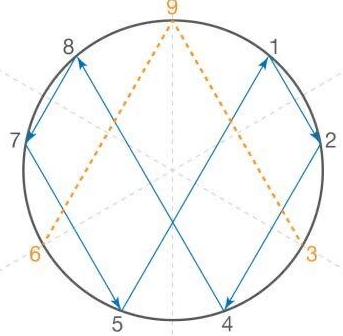
\includegraphics[width=0.38\textwidth]{./images/rsz_logo.png} \\
  \medskip
  ad infinitum \\
  
  \vspace*{1\baselineskip}
  
\includegraphics[width=0.24\textwidth]{./images/rsz_npqr.png} \\
  \vspace*{3\baselineskip}
 

\pagebreak
\endgroup
}

\newdateformat{usvardate}{%
\monthname[\THEMONTH] \ordinal{DAY}, \THEYEAR}
\newdate{DocDate}{21}{12}{2020}

\begin{document}

\title{\rmfamily\normalfont{Nexus: A New Internet Protocol}}

\date {\usvardate \displaydate {DocDate}}
\maketitle
\begin{abstract}
\bigskip


\noindent The Internet is one of the most important modern-day technologies, based on the Open Systems Interconnection (OSI) model with which there remains unresolved architectural limitations despite continued improvements.
Within this document, we outline a new architecture for the Internet that combines micro-satellites, phased array antennas, and software-defined routing to achieve a new degree of security and accessibility otherwise unobtainable under the OSI model used today.
These components are woven together throughout a global ecosystem that provides incentive for the growth of the network using economic models and game theory. 
Together they can replace the need for centralized Internet Service Providers (ISPs), limit censorship of free information, and give access to new services for users around the world.

\end{abstract}

\newpage

\tableofcontents
\newpage

\maketitlepage{Victor, BA, Hauk}
\newpage


\paragraph{\textbf{Protocol White Paper} - \textit{1.0.0} - Last Revised \today }

\epigraph{nexus: a connection or series of connections linking two or more things.}{\textit{\footnotesize{Oxford English Dictionary}}}


\section{Introduction}

After four years of architectural development, we are pleased to present the first document outlining the formal specifications for the Nexus Protocol (NP).
The NP is designed as a network driven by geometric economic models and advanced telecommunication hardware.
This paper outlines the current technologies underpinning the Internet, its inherent weaknesses, and how the NP aims to solve each of these deficiencies.
We also outline each discipline required to build a fully functioning NP, including Game Theory, Economics, and Systems Engineering.



\section{The Internet}

The early Internet was gradually born from a web of connections between large government sponsored organizations, namely 
\textbf{DARPA} \cite{Internet-History}, 
and was thus aptly named: \textbf{ARPANET}. 

\begin{figure}[h]
    \centering
    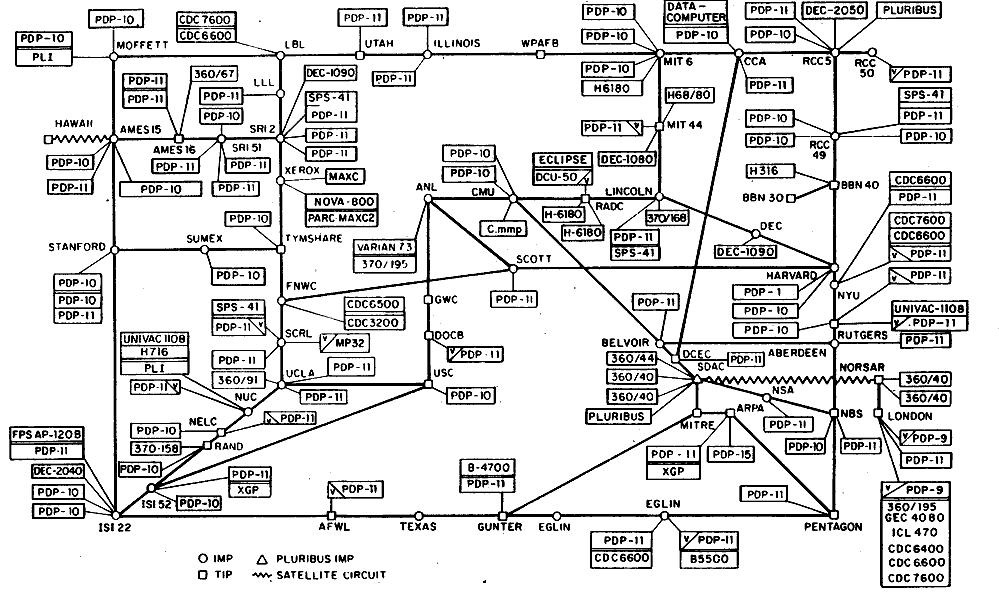
\includegraphics[width=0.80\textwidth]{./images/rsz_arpanet.png} \\
    \caption{ArpaNet Logical Map, March 1977 \cite{ARPANET}}
\end{figure}

\noindent The initial Internet routing system was a highly trusted environment between large institutions and functioned effectively before the commercialization of the technology.


\subsection{The OSI Model}

\begin{wrapfigure}[11]{r}{0.55\textwidth}
    \centering
    \vspace{-30pt}
    \hspace{0pt}
    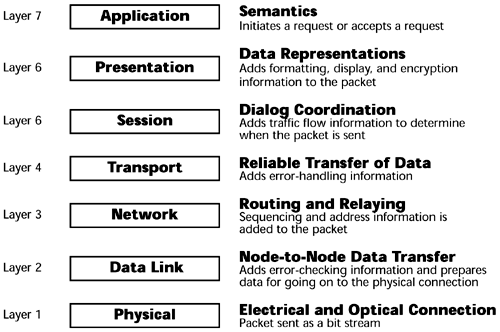
\includegraphics[width=0.55\textwidth]{./images/rsz_osi.png} \\
    \caption{The OSI reference model \cite{NetworkOSI}}
\end{wrapfigure}

The Internet is built using a conceptual blueprint of 7 layers called the ``OSI Reference Model''.
This model reflects the flow of data from Layer 1, the physical layer, through to Layer 7, the application space. 
It has served as a reference model for protocol stacks over the past three decades, enabling the creation of open standards such as Transmission Control Protocol/Internet Protocol (TCP/IP) and Hypertext Transfer Protocol (HTTP), and continues to serve as the model for IETF and IEEE standardization documents.


\subsection{Internet Protocol}

The Internet Protocol (IP) is a well-known addressing system that creates a machine-readable mapping to a physical location.
It acts as both a network \textbf{Identifier} and \textbf{Locator}, and has two main forms: IPv4 and IPv6. 
Each has a maximum number of mappings and are used by routers across the Internet to direct packets to their addressed location.
This coupling of identifier and locator results in a new network identity when changing your internet connection source, for instance moving from LTE to Wi-Fi.


\subsection{Authentication}

The OSI Reference Model authenticates on the Session Layer when using Secure Sockets Layer (SSL) with Certificate Authorities (CA's) but with the Network and Data Link Layers, they do not have authentication mechanisms in place.
This creates exploitable attack vectors whereby elements including Address Resolution Protocol (ARP) caches can be spoofed, creating a false mapping between the Data Link (MAC Address) and the Network (IP Address) layers, rendering public networks unreliable even with centralized solutions such as CA's.



\section{Network Architecture}

Outlined within the below subsections are some of the fundamental architectural components that will be needed to satisfy the Nexus Protocol's design requirements, including but not limited to antennas, operating frequencies, satellites, and ground stations.
We will outline these requirements with architecture that fulfills their needs, along with expected values for revenue, cost, and performance for select subsystems.


\subsection{Phased Array Antennas}

\noindent A Phased Array antenna is a fixed, electronically-steered antenna that can reach high enough gains and mobility for sustained two-way communication between satellites and ground stations. The following illustration shows how interference patterns are utilized to steer the beam of radio waves.

\begin{figure}[h]
    \centering
    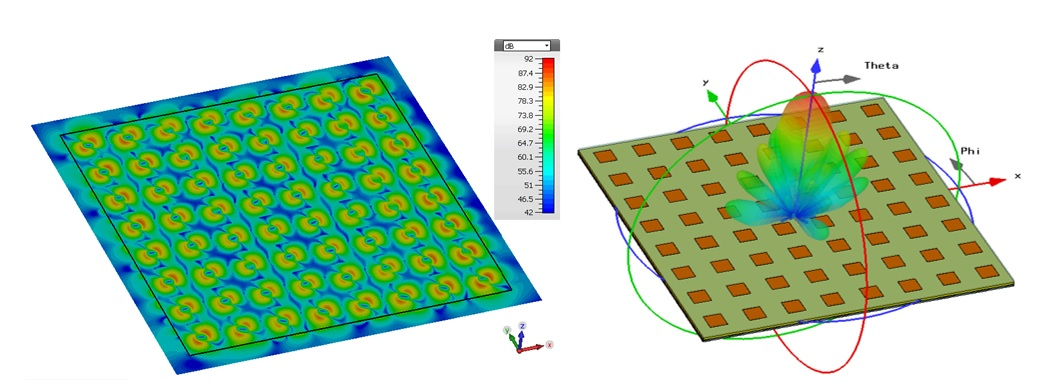
\includegraphics[width=0.9\textwidth]{./images/rsz_phased_array.jpg} 
    \caption{Phased Array Antenna (8x8) beam forming \cite{Phased-Arrays}}
\end{figure}

\subsubsection{Higher Gains}

Our link budget [\ref{3.2.2}] requires antenna gains to be above 33 dBi for reasonable data rates [\ref{3.2.3}].
Several options meet that requirement including satellite dishes, Yagi (18 dBi+), and phased array antennas.
Although a satellite dish or Yagi antenna could work, they are limited in size and maneuverability, making them less desirable for use in a highly dynamic satellite and ground routing system.
A phased array antenna is both very dynamic and able to achieve high gains, which makes it the perfect hardware to fulfill our requirements.

\subsubsection{Beam Forming}

A phased array antenna forms the beam electronically, deploying a steered beam which can track a moving satellite overhead, quickly and without physical movement.
The lack of moving parts makes this solid-state antenna extremely durable but just as important, the interference pattern that is used to steer the beam also provides excellent security properties [\ref{packet-sniffing}]. Eavesdroppers need to be directly in the path of the beam to sniff packets, otherwise they will only intercept the interference signal used to steer the radio-wave beam.

\subsubsection{Portability}

The phased array antenna size is dependent on the wavelength that is being transmitted, and the total number of elements.
A minimum number of elements is required to increase signal gains to reasonable levels while the spacing between elements is fixed (2.584 cm for 5.8 GHz).
This makes communication systems using extremely high frequencies very portable, with small antennas able to achieve gains exceeding 33 dBi.


\subsection{Frequency Allocation}

In order to meet the promise of a free and open protocol, frequency allocation must fall within internationally agreed frequency ranges for unlicensed operations.
The sections below describe the frequencies we will use for communication, including mathematical proofs of their viability.

\subsubsection{ISM Frequencies}

There is a subset of the Radio Frequency (RF) spectrum that does not require a license to use, being predetermined by the International Telecommunications Union (ITU) for unlicensed international use.
This collection of frequencies are called ISM (Industrial, Scientific and Medical) \cite{ISM_Table}, with relevant allocations listed below: 

\smallskip
\begin{table}[ht]
\begin{center}
\begin{tabular}{c|ccc|}
    \hline
    \hline
     & \textbf{Frequency} & \textbf{Bandwidth} & \textbf{Availability}\\
    \hline

    
    \multirow{4}{*}{\rotatebox[origin=c]{90}{ISM Table}}
    %&27.120 MHz & 326.0 KHz & Global \\
    &40.680 MHz & 40.00 KHz & Global \\ 
    &2400.0 MHz & 100.0 MHz & Global \\
    &5800.0 MHz & 150.0 MHz & Global \\
    &24.125 GHz & 100.0 MHz & Global \\
    
    \hline
    \hline
\end{tabular}
\end{center}
\end{table}

\noindent Without licensing requirements, they have become very popular for short range wireless communication systems such as Wi-Fi, specifically 2.4 GHz and 5.8 GHz.
This open licensing is fundamental for our new communication standards to be realized, remaining unrestricted and unowned by any single party.

\subsubsection{5725 - 5875 MHz}
\label{3.2.2}

5.8 GHz was allocated globally in 1999, to desaturate the already crowded 2.4 GHz spectrum (Bluetooth, Microwaves, WiFi, etc.).
This spectrum currently has more lenient regulations such as unlimited antenna gains, unlike the 6 dBi restriction on 2.4 GHz devices \cite{ISM_Limits}.
The primary constellation will operate at an orbital inclination of 500 km above the Earth's surface and thus require high directional gains (33 dBi+) to overcome path loss.
The following demonstrates our link budget:

\begin{center}
\newenvironment{conditions}
  {\par\vspace{\abovedisplayskip}\noindent\begin{tabular}{>{$}l<{$} @{${}={}$} l}}
  {\end{tabular}\par\vspace{\belowdisplayskip}}

\textbf{The following describes input power (dBm):}
\begin{equation}
\resizebox{.25\hsize}{!}{$P_t = 10 \cdot log(w)$}
\end{equation}
\textbf{where}:
\begin{conditions}
 P_t     &  transmitted power in Decibel-Milliwatts (dBm) \\
 w       &  input power in milliwatts (mW) \\
\end{conditions}

\textbf{which results in:} \\
\medskip
\resizebox{.35\hsize}{!}{$P_t = log(1000)$ = 30 dBm}
\bigskip


\bigskip
\textbf{The following describes free space path loss in Decibels (dB):}
\begin{equation}
\resizebox{.55\hsize}{!}{$L_{FS} = 32.44 + 20 \cdot log(d) + 20 \cdot log(f)$}
\end{equation}
\textbf{where}:
\begin{conditions}
 L_{FS}     &  free space path loss (dB) \\
 32.44      &  constant specific to units used (MHz and km) \\
 d          &  the distance to travel (km)\\
 f          &  the frequency being used (MHz) \\
\end{conditions}

\textbf{which results in:} \\
\medskip
\resizebox{.75\hsize}{!}{$L_{FS} = 32.44 + 20 \cdot log(500) + 20 \cdot log(5825)$ = 161.7\underline{3} dB} \footnote{Figures $d = 500$ km while $f = 5825$ MHz to match units for constant $32.44$}


\bigskip
\textbf{This is then combined with our gains to calculate link-budget:}
\begin{equation}
\resizebox{.75\hsize}{!}{$P_{RX}=P_{TX} + G_{TX} + G_{RX} - L_{TX} - L_{FS} - L_P - L_{RX}$}
\end{equation}
\textbf{where}:
\begin{conditions}
    P_{RX}  & received power (dBm) \\
    P_{TX}  & transmitter output power (dBm) \\
    G_{TX}  & transmitter antenna gain (dBi) \\
    G_{RX}  & receiver antenna gain (dBi) \\
    L_{TX}  & transmit feeder and associated losses (feeder, connectors, etc.) (dB) \\
    L_{FS}  & free space loss or path loss (dB) \\
    L_P   & miscellaneous signal propagation losses (weather, fading margin, etc.) (dB) \\
    L_{RX}  & receiver feeder and associated losses (feeder, connectors, etc.) (dB) \\
\end{conditions}


\textbf{which results in:} \\
\medskip
\resizebox{.65\hsize}{!}{$P_{RX} = 30 + 33 + 33 - 2 - 161.73 - 2$ = -69.73 dBm} \footnote{Figures $L_{TX} = 2$ dB while $L_{RX} = 2$ dB assuming low losses due to short feeders}
\medskip

\end{center}


\noindent The above link budget does not account for $L_P$ due to weather (moisture absorbs RF), fade margins, polarization mismatches, or other miscellaneous propagation losses. 
It demonstrates a received signal strength of $-7\underline{0}$ dBm broadcasting at 1W, having antenna gains exceeding 33 dBi for both $G_{TX}$ and $G_{RX}$. 


\bigskip
{\noindent\textbf{The Karman Line}} \\

\noindent From our understanding, regulations are only enforceable within jurisdiction which is generally accepted (and still debated) to extend to the Karman line (approximately 100 km above sea level) \cite{karman-line}.
Because of this, we suspect we may be afforded the opportunities to increase satellite transmitting power as long as received ground based signal strength does not exceed $30$ dBm.
If this proves to be true, we will be able to provide higher signal strength for downlink if power was available, reducing dependence on increasing gains.

\subsubsection{Bandwidth and Latency}
\label{3.2.3}

Using advanced modulation techniques, 5.8 GHz can provide very high bit rates with low latency, as long as the signal to noise ratio (SNR) is high enough for low error rates.

\bigskip 
{\noindent\textbf{Expected Bandwidth}} \\

\noindent As the RF spectrum saturates or link budget decreases, signal bit rate must decrease due to higher error rates in the modulation patterns.
We use 1 spacial stream ($1xSS$) for each entry in the table, to show our expected data rates per stream.
The following table data was populated with the data-sheet from modest hardware: an Aruba 510 Series Wireless Access Point \cite{data-rates}, using Modulation and Coding Scheme (MCS) tables to derive correct bit rate using a conservative symbol duration of $800 \mu S$.


\bigskip
\begin{table}[ht]
\begin{center}
\begin{tabular}{c|ccc|}
    \hline
    \hline
     & \textbf{Data-Rate} & \textbf{Sensitivity} & \textbf{Bandwidth}\\
    \hline
    
    \multirow{4}{*}{\rotatebox[origin=c]{90}{802.11n}}
    &6.5 Mbps & $-93$ dBm & $20$ MHz \\
    &13.5 Mbps & $-90$ dBm & $40$ MHz \\ 
    &65 Mbps & $-73$ dBm & $20$ MHz \\
    &135 Mbps & $-70$ dBm & $40$ MHz \\    
    \hline
    
    
    \multirow{4}{*}{\rotatebox[origin=c]{90}{802.11ac}}
    &27 Mbps & $-87$ dBm & $40$ MHz \\
    &58 Mbps & $-84$ dBm & $80$ MHz \\
    &180 Mbps & $-65$ dBm & $40$ MHz \\ 
    &390 Mbps & $-62$ dBm & $80$ MHz \\    
    \hline
    
    
    
    \multirow{4}{*}{\rotatebox[origin=c]{90}{802.11ax}}
    &35 Mbps & $-84$ dBm & $80$ MHz \\ 
    &72.1 Mbps & $-81$ dBm & $160$ MHz \\
    &600 Mbps  & $-54$ dBm & $80$ MHz \\
    &1200 Mbps  & $-51$ dBm & $160$ MHz \\
    
    \hline
    \hline
\end{tabular}
\end{center}
\end{table}


\noindent The 802.11ax standard supports up to 160 MHz bandwidth with 8 spacial streams (8xSS), which results in a maximum bandwidth of 9.6 Gbps \cite{MCS-Table}.
This data rate requires at least $-51$ dBm receiver sensitivity (to use \textbf{1024-QAM}), realized by increasing combined antenna gains by $18$ dBi, or adding $18$ dBm to broadcasting power depending on regulatory exploration.
We expect to find similar results on data rate saturation, but with a higher error rate and thus lower bandwidth depending on circumstances such as weather, satellite hardware, and mobile ground stations such as moving vehicles. \\


{\noindent\textbf{Aggregated Bandwidth}} \\

\noindent If further bandwidth is desired, a ground station and satellite could enter into a contract that establishes exclusive access to designated ground cells [\ref{3.4.3}], creating a market for high-bandwidth connections (9.6 Gbps ideal maximum bit rate per satellite).
This hosting contract would be included as part of the Content Delivery Network (CDN) revenue outlined in section [\ref{ground-caching}], being vital to compete with available bandwidth and latency standards from centralized ISPs.

\bigskip
{\noindent\textbf{Expected Latency}} \\

\noindent At an orbital inclination of 500 km and approximating the electromagnetic (EM) propagation speed at 300,000 km/s, we can calculate the round trip time for a packet from ground station to satellite:

\begin{equation}
\resizebox{.55\hsize}{!}{$t = \mathlarger{\frac{1000}{300,000}} = 0.0033 $ seconds or $3.3 $ ms}
\end{equation}

\noindent Equation (4) displays latency is a best case scenario, where the requested data is within 500 km of the ground.
If the data is on a satellite cluster on the other side of the globe, we need to adjust for the circumference of the earth ($40,007.863$ km):

\begin{equation}
\resizebox{.55\hsize}{!}{$t = \mathlarger{\frac{41,007.86}{300,000}} = 0.137 $ seconds or $137 $ ms}
\end{equation}

\noindent Equation (5) assumes a worst case scenario where data needs to be retrieved from the host, in the absence of local ground-based caching.
These figures do not take into account computation time or serialization delays between satellites, so latency can fluctuate depending on the satellite and ground routers.
After initial data retrieval in $137$ ms, data becomes cached at the ground station and latency would reduce to 1-3 ms per locality.


\subsection{Micro-Satellites}

Micro-satellites are at the same stage of adoption as the personal computer by average consumers in 1980, with limited economic incentives and justification outside niche implementations.
An orbital network will provide direct economic incentives for deployment entities, similar to how mining has incentives in blockchain applications.
Network hardware can self-organize and deploy according to these incentives, providing unrestricted growth by decentralizing management of capital.
Further documentation will provide information on our selection of orbital inclination, minimum satellite constellation size for an initial ring network, and constellation simulations that will reinforce our expected bandwidth and latency.
This subsection will outline the value proposition for micro-satellites as part of the Nexus Protocol.


\begin{figure}[h]
    \centering
    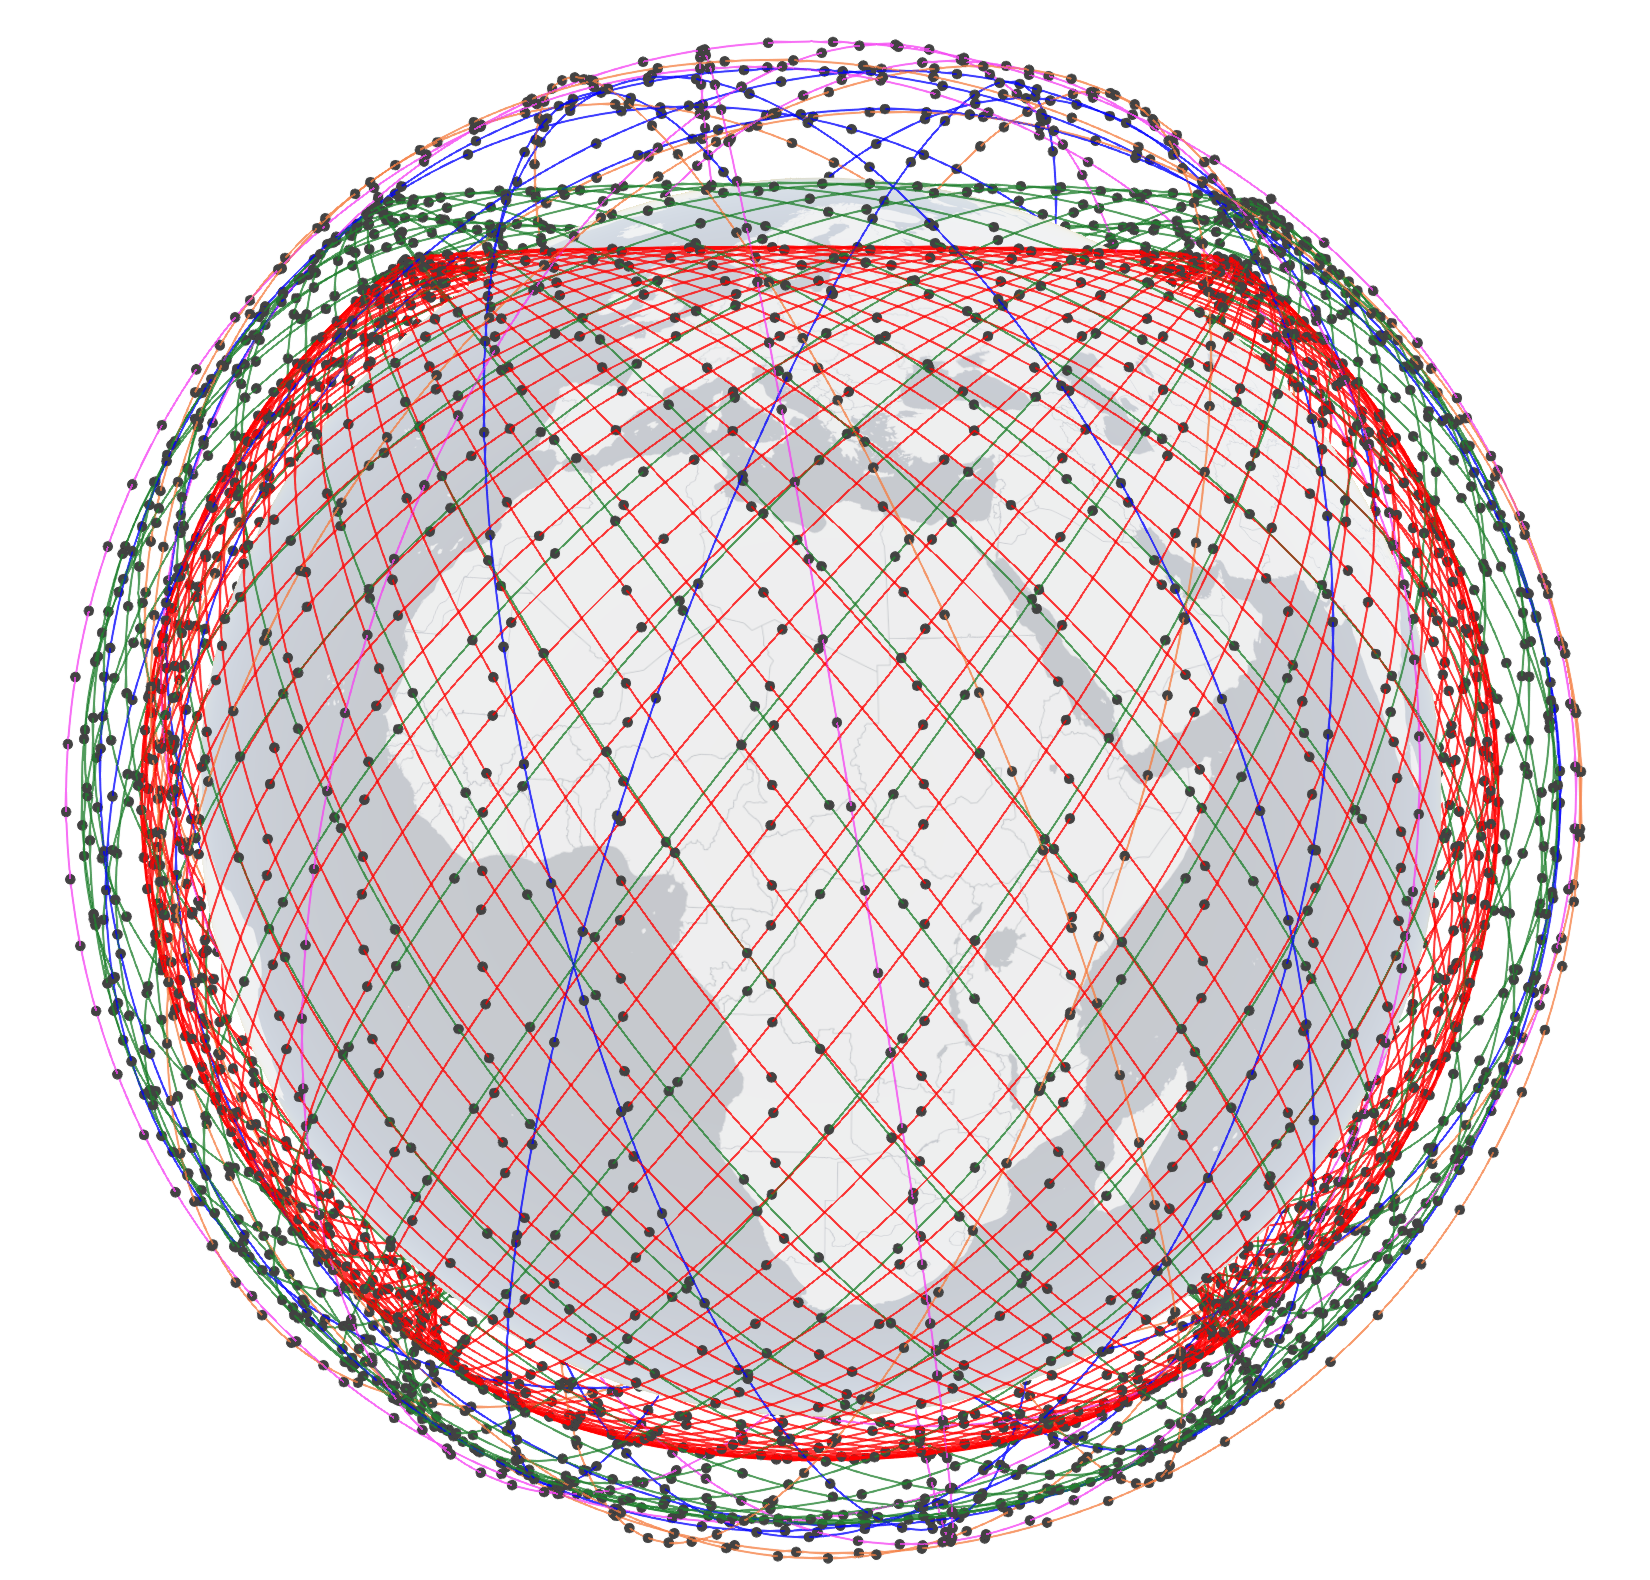
\includegraphics[width=0.8\textwidth]{./images/rsz_starlink.png} 
    \caption{Simulation of Starlink Orbital Patterns \cite{starlink}}
\end{figure}


\subsubsection{Securing Data}

One of NP's more significant value propositions is the provision of an isolated data layer for storage of sensitive information.
This data layer will be an extension of the LLD filesystem currently under development that allows individuals to negotiate hosting contracts with one another and generate direct Return on Investment (ROI) from spare storage and devices. \\

{\noindent\textbf{Design Requirements}} \\

\noindent This filesystem will be extended to encompass the orbital networks, creating a secure platform for sensitive file storage with the following advantages:

\begin{enumerate}
    \item \textbf{Immutability:} Secure data with checksums and integrity verification.
    \item \textbf{Redundancy:} Provide secure storage space for ground services and CDN's.
    \item \textbf{Development:} Store application state such as data from experiments, imaging, or weather observations.
\end{enumerate}

\noindent The orbital filesystem will integrate into the Operating System [\ref{LX-OS}] as an extension of its local filesystem, creating a common interface for managing ground and orbital based content.
This will provide easy access to space-based services and create new value propositions beyond the Internet's current realization. 
One notable example is providing direct incentives into the deployment of hardware, creating new opportunities for people to be connected and thus expand ($n^2$) the economic value [\ref{exponential-value}].
We anticipate the full realization of this vision to buffer failing economies, giving people opportunity where there was none before.


\subsubsection{Network Services}

\noindent Micro-satellites will provide reputation-based network services to supplement the routing system between ground stations and their aggregated clients.
These services rely on ground stations to shard the mapping state while maintaining a small data-set of aggregated mappings between clients and ground stations.

\bigskip
{\noindent\textbf{Design Requirements}} \\

\noindent Network services ensure continued operation of ground-based nodes, routing and caching active mappings to optimize active route bindings.
The following list expresses our design requirements, which the network service subsystems will need to fulfill:

\begin{enumerate}
    \item \textbf{Routing:} Satellite-based routing services for continued operation of other ground-based nodes.
    \item \textbf{Efficiency:} Bloom Filters \cite{bloom-filters} can be used for mapping lookups to reduce the footprint of aggregated mappings on terrestrial networks i.e. 1024 clients could be aggregated into 1 KB shared by 3 or 4 ground stations.
    \item \textbf{Mappings:} Wide Radius Locators (WRL) need to be maintained for ground station bloom filters, aggregating client mapping state while allowing non-cached mapping lookups to geo-located cell.
\end{enumerate}


\pagebreak
{\noindent\textbf{Compressed Mappings}} \\

\noindent The mapping system must allocate resources to track associations between ground station coordinates and Endpoint Identifiers (EID).
This compressed mapping state will relieve requirements on the constellations' Global System Memory (GSM), saving the larger Geo-Spacial Locator (GSL) mapping state for local ground based environments.
This compressed state can be indexed as a Geo-Spacial Distributed Hash Table (DHT) for scalability, along with saving active (EID $\longmapsto$ GSL) and (EID $\longmapsto$ WRL) mappings within available GSM.
Creating Geo-Spacial Shards (GSS) bounded to WRL's, we would require 256 MB of GSM to manage 1 Billion ($10^{9}$) devices per shard (assuming 4 stations per bloom filter, 1024 clients per cell).
An intended by product of this design is to protect against privacy leakage [\ref{privacy-leakage}], by aggregating GSL's behind orbital WRL bloom filters making it only a physically local state.



\subsubsection{Additional Services}
\label{additional-services}

\noindent A constellation's technology stack is not limited to the aforementioned services. Additional services can be built to provide a broad array of functionality to each satellite's Software Development Kits (SDK).
These supplemental services act to further reinforce the economic valuation of a given constellation, driving greater consumer demand for both the data and extended services. 
Some services could be: 

\begin{enumerate}
    \item \textbf{Imaging:} Advanced Imaging services, for generating user data.
    \item \textbf{Database:} Shared database clusters, providing a reliable and shared database service.
    \item \textbf{Sensory:} External sensory data related to astrophysics, localized planetary movements, etc.
\end{enumerate}

\noindent A service could be developed to provide new technologies enhancing external sensory data, for developers to add orbital data and sensory input into their applications.
There are many more opportunities to build upon this foundation than we have mentioned, we are just beginning to touch the surface of the possibilities.


\subsubsection{Expected Costs and Revenue}
\label{satellite-revenue}

\noindent To maximize ROI, each satellite is designed to minimize operating expenses and tap unused resources in generating revenue.
With satellites acting as a data layer, they will contain flash memory that can be leased to service providers at a given cost per byte.
Satellite constellations are designed for inter-operability, enabling constellations to specialize its services and then lease these to consumers.
The ROI will depend on the initial expense of the satellite, running costs against the available storage that can be leased on a monthly basis, and revenue generated from additional services provided by the constellation [\ref{additional-services}].
If the satellite cost is \$250k United States Dollar (USD) and it has an orbital lifespan of 5 years, it will need to achieve \$75k USD yearly revenue ($R$) for a 50\% profit margin.

\begin{equation}
\resizebox{.65\hsize}{!}{$\mathlarger{\frac{R}{S}} = \mathlarger{\frac{75,000}{1,000,000}} = 0.075$ USD per MB per year}
\end{equation}
\bigskip

\noindent The above Equation (6) displays a basic \textbf{estimate} to reference the potential costs and revenues for both consumers and operators; by no means should it be considered the actual costs.
We assumed there was no competition for the space, no additional services, and that there was 1 TB ($S$) on-board flash memory available.
If one chooses to have redundancy by engaging in multiple automated hosting contracts, this cost could be up to \$1 USD per replicated MB i.e. for 10 replications you would pay \$0.75 USD per MB per year.
All payments for terrestrial caching and orbital hosting will be made in NXS with distribution [\ref{tokenized-satellites}] and replication handled automatically.

\bigskip
\subsection{Ground Stations}

Ground stations will be responsible for doing most of the heavy processing due to supplying their localized area with content, edge computing, and routing services.
Below we will describe their requirements and functions.

\subsubsection{Managing Content}

Ground stations will be responsible for caching files that are frequently requested by its local cell.
This functionality in terms of the Internet, would be called CDNs.
The following outlines the requirements for the caching subsystem.

\bigskip
{\noindent\textbf{Design Requirements}} \\

\noindent Satellite constellations will manage files that are part of Peer to Peer (P2P) hosting contracts.
The ground infrastructure must keep current caches, adhering to the following requirements:

\begin{enumerate}
    \item \textbf{Caching:} Ground stations provide geo-located caching services for files in their local areas.
    \item \textbf{Subscribe:} Ground stations subscribe to blockchain entries updating local cache when file registers change state.
    \item \textbf{Revenue:} Ground station operators sell caching allocations to service providers following a CDN revenue model.
\end{enumerate}

\bigskip
{\noindent\textbf{Ground Station Caching}} \\
\label{ground-caching}

\noindent The ground infrastructure will be managing local data access by subscribing to file registers in order to reduce the bandwidth required and maintain the correct ground based state.

\begin{figure}[h]
    \centering
    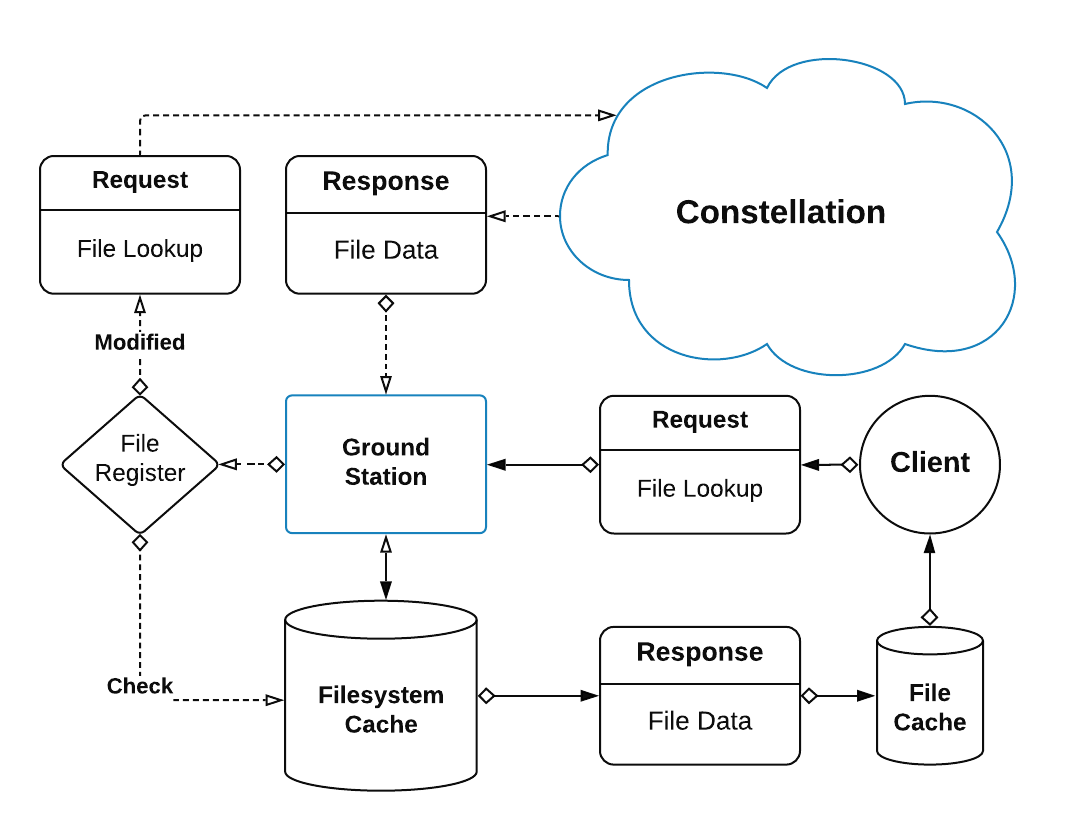
\includegraphics[width=0.85\textwidth]{./images/rsz_ground_caching.png}
    \vspace{-10pt}
    \caption{Ground Based Caching Architectural Diagram}
\end{figure}

\noindent As you can see, most of the data delivery will occur over the ground based networks, with caches that prioritize locality in the distributed system.
The File Register above is used to determine if the cache is out of sync, and requires communicating with the satellite constellation to refresh.

\bigskip
{\noindent\textbf{Generating Revenue}} \\

\noindent The ground infrastructure will provide important content delivery for local networks, creating the possibilities for owners to generate revenue and thus ROI.
With this network being designed as an immutable public access network, we want the basic use of it to be free.
This is achieved by allowing businesses and consumers to pay ground stations as CDN's, for a set amount of geo-located cache used for quicker delivery of their services and thus a better experience for their consumers. 
CDN's are projected to reach 252 ExaBytes (EB) or $252 \cdot 10^{18}$ bytes per month \cite{CDN-usage} on the current internet, so it's safe to say that there is an increasing demand for localized CDN's.
Providing this for IP/NP traffic will drive revenue to ground station operators, while being able to rely on Network Reputation [\ref{network-reputation}] for access control to remain as a free and open routing system.
\bigskip


\subsubsection{Aggregated Mapping}
\label{aggregated-mapping}

\noindent The mapping system relies strongly on ground infrastructure to shard and aggregate the mapping state.
This is a key component to providing a globally accessible mapping system, that handles lookups between ground stations, enhancing the privacy and security of the networks.

\bigskip
{\noindent\textbf{Design Requirements}} \\

\noindent The following list describes our primary design requirements for aggregated mapping systems.
They cover fundamental privacy and scaling qualities by offloading mapping to ground stations to realize a globally scalable mapping system.

\begin{enumerate}
    \item \textbf{Scaling:} Mapping for billions of devices is not feasible as an orbital state.
    \item \textbf{Privacy:} Globally available GSL's for individual EID's creates privacy vulnerabilities, thus we need to take advantage of locality.
    \item \textbf{Routing:} Ground Stations must handle Re-Encapsulating packets, to strip off ground station locators for client's registered locators.
\end{enumerate}

\bigskip
{\noindent\textbf{Re-Encapsulating Locators}} \\

\noindent In terms of the Locator-ID Separation Protocol (LISP) \cite{LISP}, there is an architectural component called the Re-encapsulating Tunnel Router (RTR). 
This is responsible for re-encapsulating packets to their final destination and port, if they happen to be aggregated behind Network Address Translators (NAT).
Ground stations will follow a similar principle, operating with a local mapping state that aggregates behind ground stations, allowing a sufficient client per ground station ratio.
Packets will be addressed to identifiers, and encapsulated with locators.
Ground stations will re-encapsulate by performing a local map-cache lookup, then re-transmit the packet with the updated locators to designated ground cell.
The stratification of the overlay network for its division into separate local systems with independent mapping systems is described in detail in draft-moreno-lisp-uberlay \cite{uberlay}.

\begin{figure}[h]
    \centering
    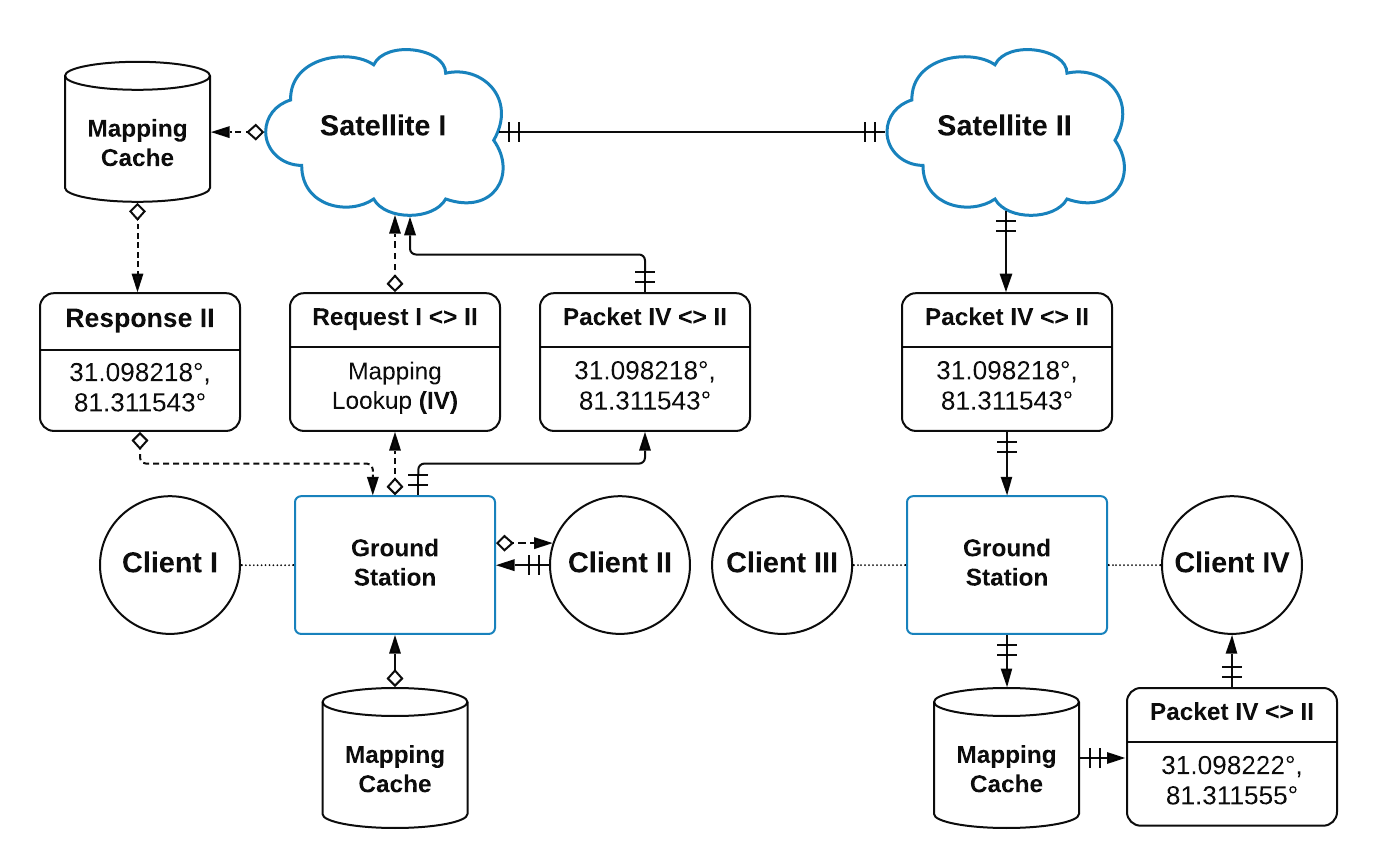
\includegraphics[width=1\textwidth]{./images/rsz_re_encapsulating.png}
    \caption{Mapping Lookup and Re-Encapsulation Architectural Diagram}
\end{figure}

\begin{center}

\end{center}

\noindent As illustrated in the diagram above, the mapping lookup is done for the ground station through the satellite's mapping cache, existing in compressed form.
This is then used to lookup the WRL to find the ground station serving the destination EID.
Once these locators are known, sent from EID (II) to EID (IV), this packet is routed to the correct satellite which down-links to the ground station.
The packet is then re-encapsulated with the EID's local GSL, completing the route to EID (IV).


\subsubsection{Cell Topology}
\label{3.4.3}

The ground infrastructure will follow a cell-like topology, acting as an aggregation service and reducing the overall RF saturation.
Mesh networks have broken down at high usage in densely populated areas due to large RF saturation caused by isotropic radiators and current IP (Internet Protocol) designs.
Our architecture is looking to solve these saturation and routing issues by reducing the overall isotropic radiation through high gain, directional phased array antennas. 
This cell topology also provides us with crucial aggregation and caching characteristics that become valuable in ensuring the protocol and mapping system scale.

\begin{figure}[h]
    \centering
    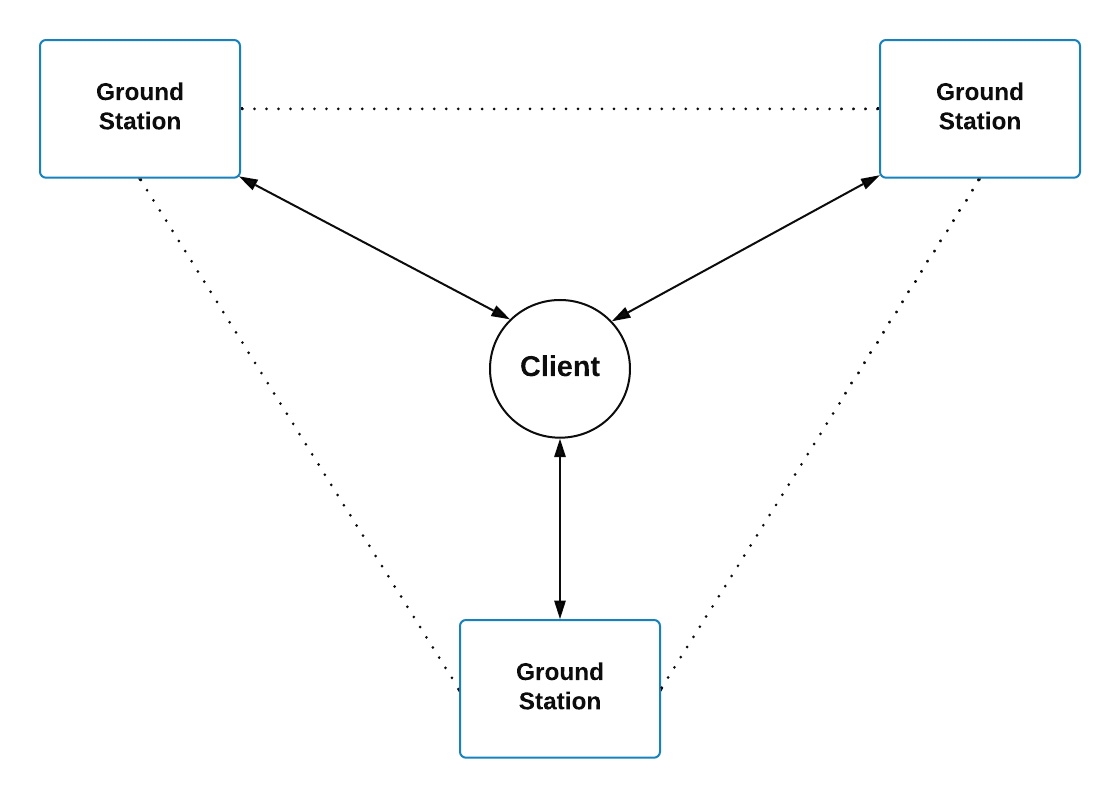
\includegraphics[width=0.7\textwidth]{./images/rsz_triangulation.png}
    \caption{Signal Triangulation and Cell Topology}
\end{figure}

{\noindent\textbf{Signal Triangulation}} \\ 

\noindent Signal triangulation supplies additional input for GSL registration in the local mapping system, allowing operation of clients that do not have access to GPS chips.
Both GPS and signal triangulation can be combined when available to utilize an average coordinate for more precise GSL mappings.



\subsubsection{Interoperating}

In order for the NP to provide the proposed access, the ground stations need to interoperate with existing hardware in as many ways as possible.
We are currently exploring options to adopt either one of the two standards mentioned below for ground infrastructure.

\bigskip
{\noindent\textbf{802.11 Requirements}} \\

\noindent This first list describes our requirements for maintaining security focused 802.11 links from ground stations to clients:

\begin{enumerate}
    \item \textbf{Ground Wi-Fi:} 802.11 can be used to provide local hot-spots at ground stations.
    \item \textbf{Authenticate:} In order to be safely used as public Wi-Fi's, ARP and DNS (Domain Name Service) cache modifications must be authenticated. We are assessing candidates such as S-ARP \cite{S-ARP} to provide authentication mechanisms.
    \item \textbf{Range:} Excessive RF saturation exists at 2.4 GHz and antennas have limitations of 6 dBi gain so we will focus on the 802.11 protocols that rely on 5.8 GHz for higher gains and thus range.
\end{enumerate}

{\noindent\textbf{LTE Opportunities}} \\ 

\noindent The next list describes our opportunities for ground station compatibility with LTE clients, while also maintaining a security focused approach:

\begin{enumerate}
    \item \textbf{Cellular:} LTE technology can potentially be used as another access point to ground stations.
    \item \textbf{Licenses:} Some frequencies for LTE are publicly available ISM bands.
    \item \textbf{Roaming:} Potentially backwards compatible data roaming with legacy cellphones and mobile devices.
\end{enumerate}




\section{Operating System}
\label{LX-OS}

LX-OS, which stands for [\textbf{L}][\textbf{L}ower \textbf{L}evel \textbf{L}ibrary, \textbf{L}4 Microkernel, \textbf{L}ISP] $\longmapsto$ [\textbf{X}][Ne\textbf{X}us] $\longmapsto$ [\textbf{OS}][\textbf{O}perating \textbf{S}ystem], has strong security requirements to reduce the overall risk of embedded devices, cube satellites, and consumer grade hardware.
We intend to enforce these security qualities by reducing the local attack surface through the use of cryptographic authentication and verification from a common ledger of truth, provided by Nexus.
The following subsections will outline our design requirements, technical architectures, standards and concepts that will be implemented in LX-OS.



\subsection{Design Requirements}

When a device comes online, rather than utilizing conventional superuser/guest architecture like most monolithic kernels provide, changes to critical areas of the user-space will require user generated cryptographic proofs to be validated.
This ultimately reduces the attack surface from the local device's state, while simultaneously providing ancillary services to the developer and consumer.
The following list expresses our design requirements:

\begin{enumerate}
    \item \textbf{Resistance} to most common exploits, including buffer overflow.
    \item \textbf{Protection} against insecure applications in shared environments.
    \item \textbf{Redundancy} and integrity checking on local and remote filesystems.
    \item \textbf{Routing} and forwarding as a software defined service for both IP/NP.
    \item \textbf{Decoupling} of hardware and user-space, i.e. virtual user-space.
    \item \textbf{Framework} for deploying high security embedded devices quickly.
\end{enumerate}

\bigskip
{\noindent\textbf{Hardware Compatibility and Integrity}} \\

\noindent The initial hardware for the OS design is targeted for satellites and IoT devices, however only a small range of platforms will be supported early. 
Due to the increasingly questionable integrity of the hardware industry the selection for the correct hardware is still under investigation. 
Several open source platforms including RISC-V are under consideration and will be reviewed for initial support respective to its viability in the aforementioned network architecture.

\bigskip
{\noindent\textbf{Micro-kernels}} \\

\noindent A micro-kernel is not a new concept, but it has taken many decades to mature to a point where it could compete with its monolithic counterparts. 
Most of the operating systems on the market today use either a monolithic or hybrid kernel model, meaning that complexities such as file-systems, network communication, and memory policies are all handled in the kernel.
Some of the downsides of monolithic and hybrid kernel designs is lack of robustness, as one failure in any kernel subsystem will require the entire system to be rebooted to a clean state.

\begin{figure}[h]
    \centering
    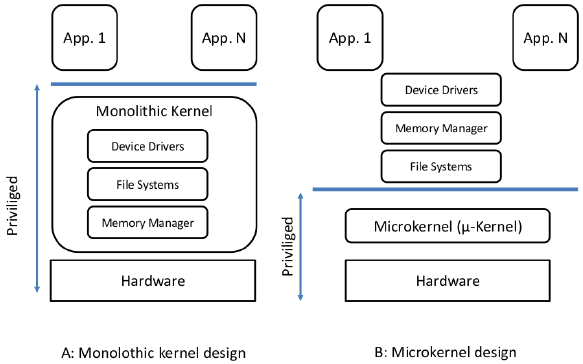
\includegraphics[width=0.8\textwidth]{./images/rsz_mono_micro.png} 
    \caption{Monolithic vs Micro-kernel Architectural Comparison \cite{kernel-architecture}}
\end{figure}

\noindent Though monolithic kernels have come a long way with the likes of Linux, they still have many vulnerabilities that can put the entire system at risk from one faulty component or driver.
This is why in order to meet our design requirements, we will focus efforts towards improving micro-kernel performance comparable with their monolithic counterparts.


\subsection{Memory Protection}

Using the correct memory policies, when developed at the operating system level, one can overcome many of the limitations and security precautions of development including buffer overflow exploits.
We achieve this by combining together memory policies from seL4 (Secure L4) \cite{seL4} with additional components that strengthen protection even further.

\begin{figure}[h]
    \centering
    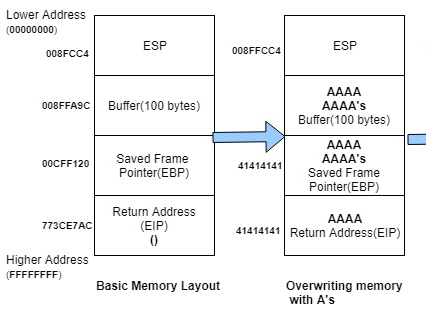
\includegraphics[width=0.7\textwidth]{./images/rsz_buffer_overflow.png}
    \caption{Overwriting Memory with Buffer Overflow \cite{buffer-overflow}}
\end{figure}

\noindent The above diagram illustrates how a buffer overflow exploit operates, by overwriting critical parts of run-time memory that allows injection of arbitrary code without user action.
This is a type of exploit deployed by many worms, viruses and similar malware to establish Advanced Persistent Threats (APT) across the internet that most modern day operating systems have very few protections against. 
Generally a buffer overflow exploit occurs from a bug in a running application, that can be exploited to compromise the entire system.
The next sections will outline how we are able to overcome conventional buffer overflow exploits, using strict memory policies inherited through seL4, along with run-time verification of process memory.


\subsubsection{seL4 Memory Verification}

seL4 is a micro-kernel with unique memory protection design principles, particularly formed through the usage of new memory management objects, creating stronger guarantees that run-time memory allocated to a specific process cannot cross isolation boundaries. 
seL4 has already been proven in the wild to stop similar attacks, having been battle tested on military drones to thwart threat actors.
It is a formally verified micro-kernel, meaning that mathematical proofs can be generated to ensure that the kernel operates as designed, or is as close to bug-free as possible.

\begin{figure}[h]
    \centering
    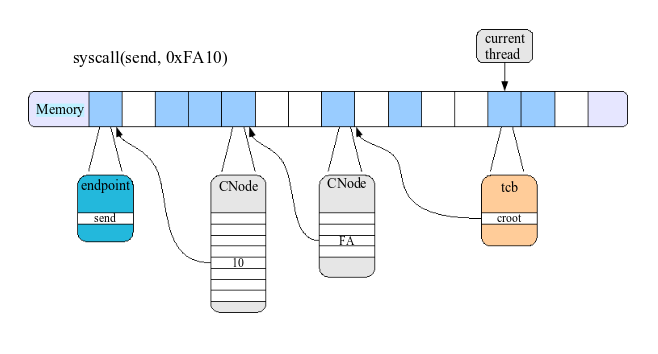
\includegraphics[width=0.9\textwidth]{./images/rsz_syscall.png}
    \vspace{-20}
    \caption{seL4 System Call Memory Layout Diagram \cite{seL4-syscall}}
\end{figure}

\bigskip
{\noindent\textbf{Isolation of Components}} \\

\noindent seL4 has unique isolation qualities that ensures that processes cannot access each other's memory, which is a strong requirement for system security.
The resource manager will be integrated with Nexus, ensuring that any changes in state that require a user action are cryptographically authenticated before being executed by the system. 

\begin{figure}[h]
    \centering
    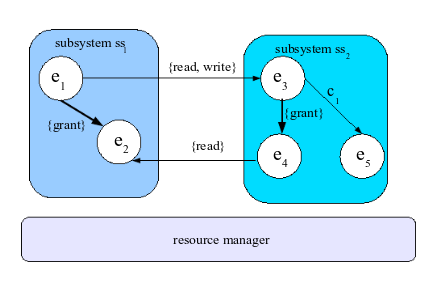
\includegraphics[width=0.6\textwidth]{./images/rsz_isolation.png}
    \vspace{-20}
    \caption{Process Memory and Process Isolation Diagram \cite{seL4-syscall}}
\end{figure}

\noindent This above resource manager will be responsible for helping maintain LX-OS isolation requirements, giving strong guarantees that one process cannot gain authority over another.
These seL4 mechanisms provide additional tools to protect LX-OS memory thus minimizing the memory related attack surface.


\subsubsection{Protecting during Runtime}

\noindent LX-OS will keep checksums of stack and heap allocations, specifically for critical subsets of the aforementioned memory zones.
This provides us additional run-time protection, in case the previous isolation characteristics are penetrated giving us additional redundancy and protection.
The following list describes LX-OS run-time process:

\begin{enumerate}
    \item \textbf{Merkle Trees:} Memory zones hold checksums as pages or blocks of memory that contain merkle paths of related states.
    \item \textbf{Critical:} Stack pointers and critical system values that the OS relies on must be hashed to ensure critical system components cannot be tampered with.
    \item \textbf{Allocation:} To receive new memory allocations from the resource manager, an authenticated user action must be performed. This could be as cached credentials for automated authentication if pre-allocated, or a user specified manual action (i.e. ulimit).
\end{enumerate}

\noindent With the aforementioned techniques and supporting documentation, we can achieve a strong guarantee of isolation between components and run-time memory protection, thus satisfying an LX-OS design requirements for protection against most OS level exploits.
We believe seL4 with its formally verified micro-kernel is the best option to fulfill our long term vision, and a great foundation to build LX-OS from.

\subsection{Filesystem}

The filesystem will manage multiple dynamic requirements to ensure integrity of the core system.
It will operate as a distributed filesystem, giving developers a common POSIX interface for working with files in the filesystem.
The filesystem will have verification on a per block level, while handling paging from distributed information sources. 
The following will outline these key integration structures, and how they will be achieved with the NP network architecture.

\subsubsection{Integrity Verification}

\noindent One significant flaw in most OS level designs, is the ability for a remote program to inject itself into existing files, making it difficult to detect within a filesystem.

\pagebreak
\noindent Below we explain how integrity checking will function, and how this will protect the entire system from intrusion of unauthorized programs.

\begin{enumerate}
    \item \textbf{Integrity:} Filesystem integrity checking using blockchain registers, with both cypher-text and plain-text checksums.
    \item \textbf{Immutable:} Filesystem metadata, paths and directory structure managed through the use of Nexus.
    \item \textbf{Assurance:} This ensure integrity even with distributed hosting, and protects the filesystem from tampering by remote attackers.
\end{enumerate}

\begin{figure}[h]
    \centering
    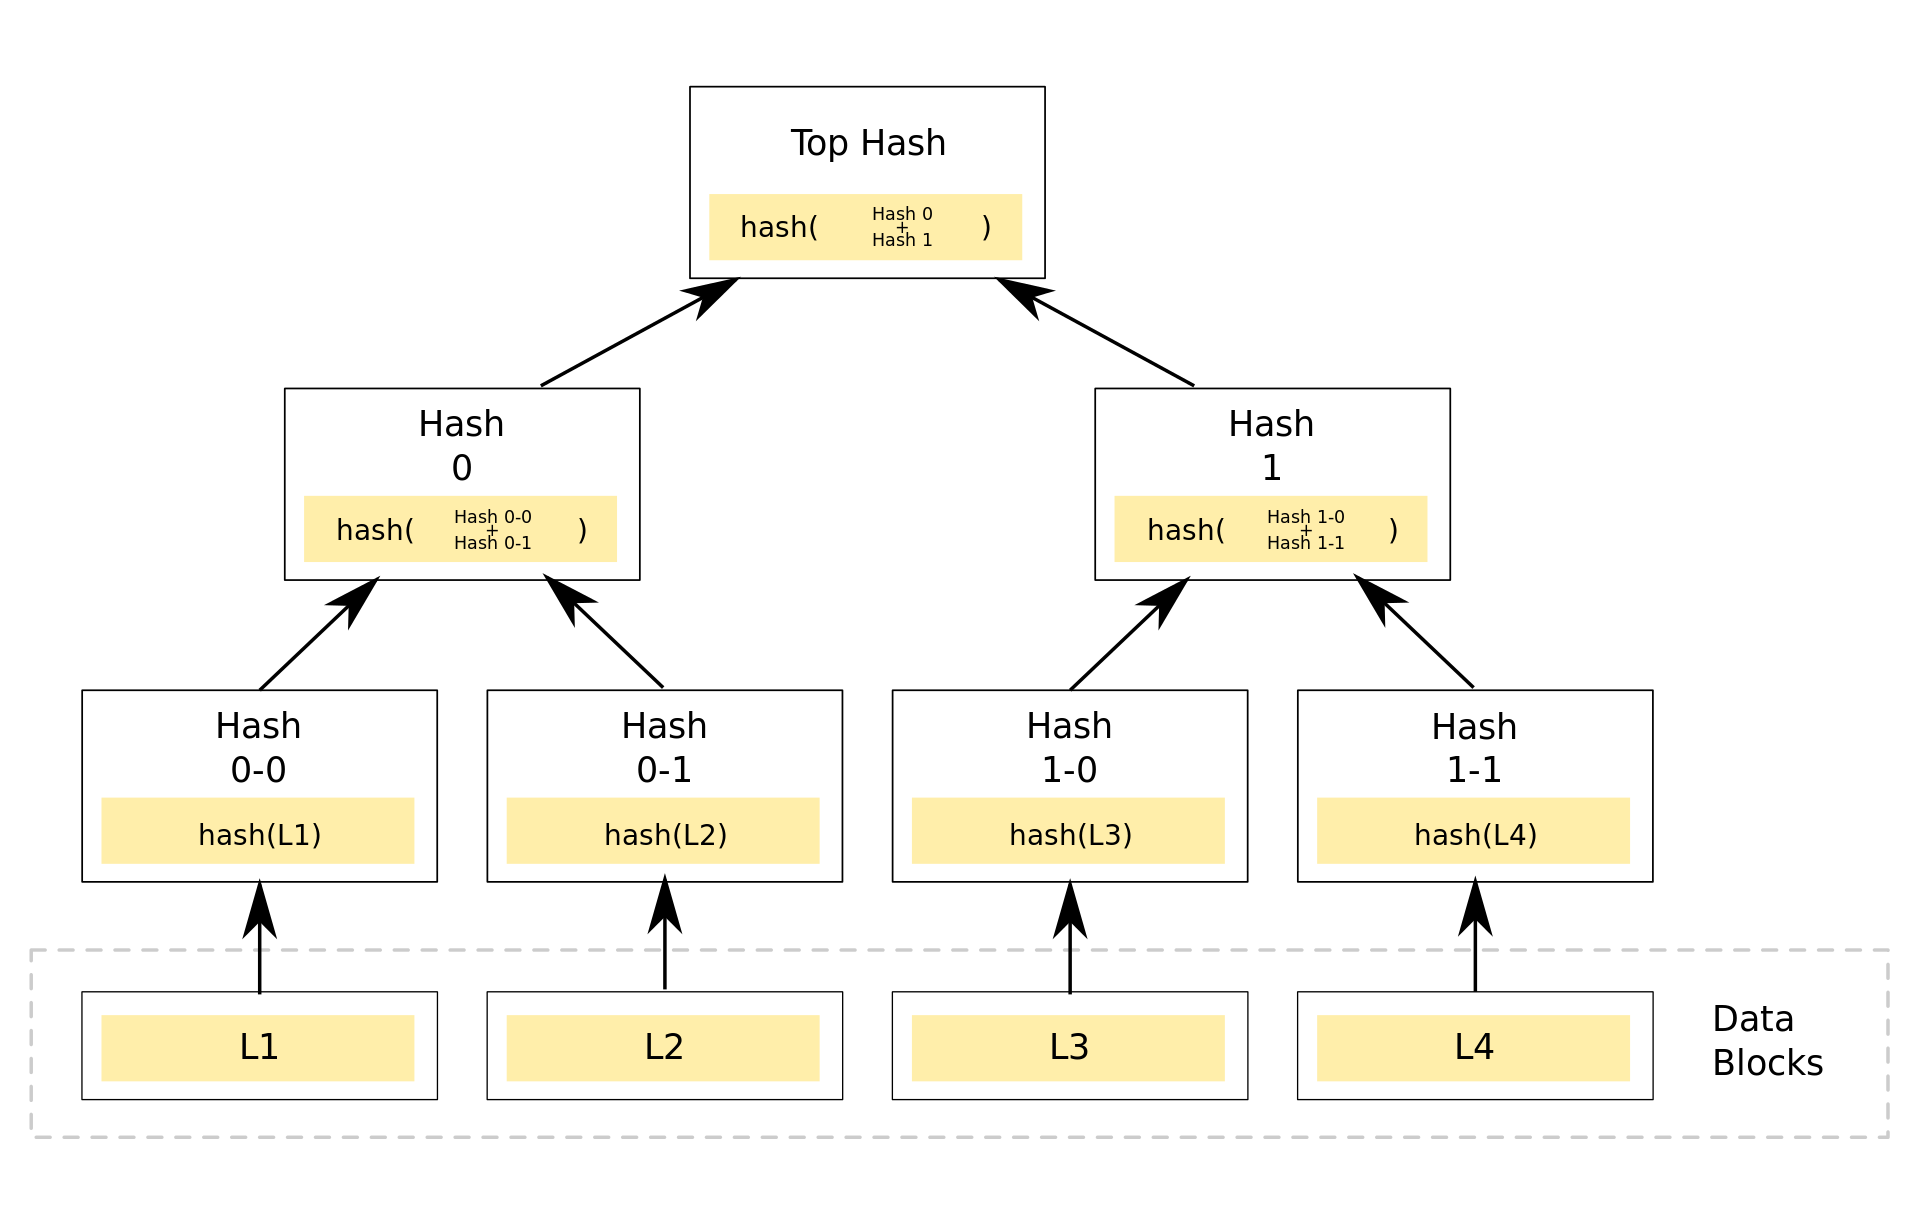
\includegraphics[width=0.85\textwidth]{./images/rsz_merkle.png}
    \caption{Merkle Tree Composed of Four Nodes \cite{merkle-tree}}
\end{figure}

\noindent The above diagram illustrates a merkle tree, using L1, L2, L3, and L4 as blocks of the individual file, and the Top Hash being what is stored in the file register.
This serves multiple purposes, including creating immutability and a signalling system for ground based caching [\ref{ground-caching}].

\subsubsection{Distributed Paging}

Paging can be done in a distributed fashion so that all computers servicing sub networks will see each other as separate components of the same system. 
Ground System Caching [\ref{ground-caching}] will also be a fundamental element in distributed paging, as a page fault will be handled by making a lookup to the appropriate constellation if all ground infrastructure is without a viable cache.
This makes the satellite network the final step in handling page faults, which seamlessly integrates into the OS as illustrated in the diagram below:

\smallskip
\begin{figure}[h]
    \centering
    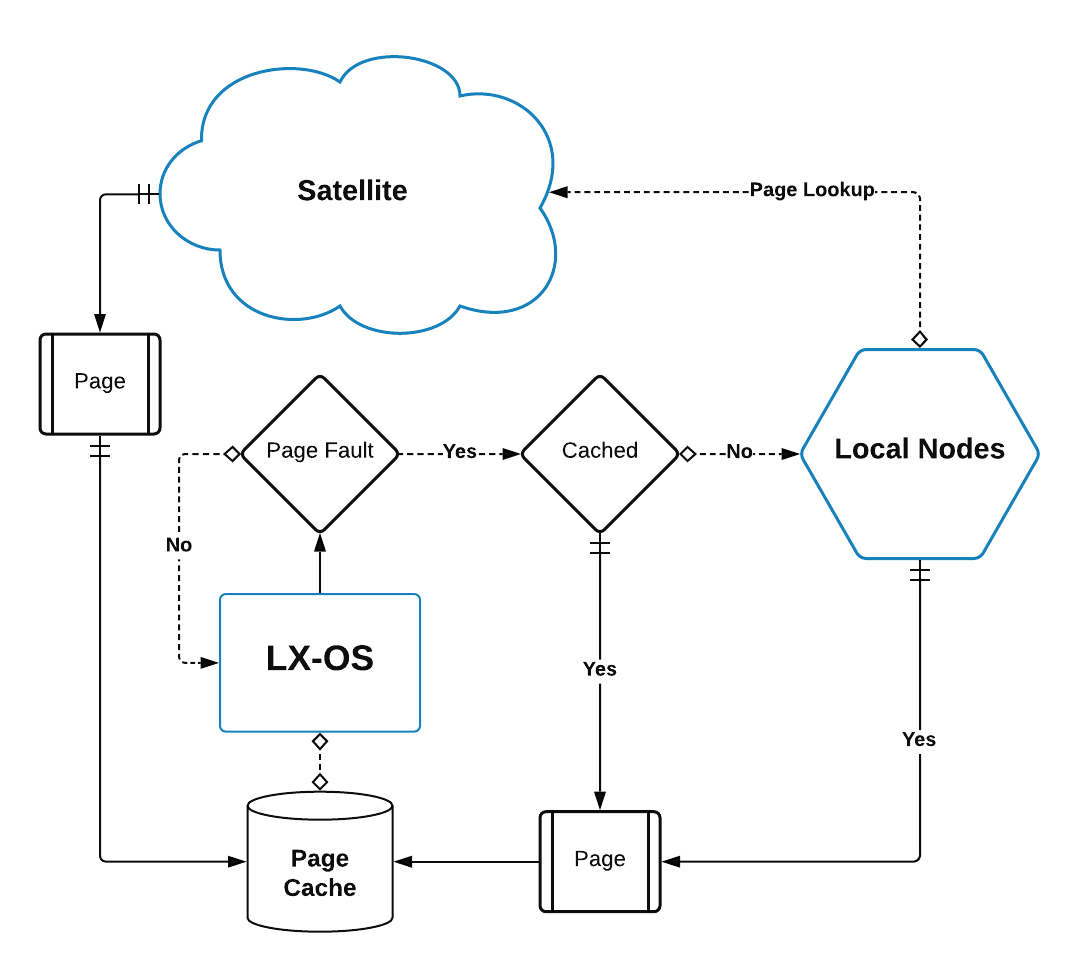
\includegraphics[width=0.9\textwidth]{./images/rsz_page_fault.png}
    \caption{Distributed Page Fault Architectural Diagram}
\end{figure}

\noindent Building on LX-OS will be similar to developing on Linux, with the magic happening below the application space so that developers are not burdened with additional complexities, automating the distributed lookups.


\subsection{Software Defined Routing}
\label{software-routing}

The Internet as we know it is mostly hardware defined meaning that in order to enhance functionality in routing systems one needs to buy new hardware.
The architecture of NP is based on software defined routing so that systems can be upgraded without requiring purchase of additional hardware (i.e. IPv6 is still is not fully adopted after two decades).
The business model of artificial hardware lifespans is already reaching its limitations and thus software defined services will become more predominate as a potentially resource constrained future will create greater requirements for efficiency and utilization of hardware.


\subsubsection{Separating Locators and Identifiers}

The NP addressing system relies on LISP to maintain isolation between locators and identifiers.
This allows inter-operation with other Routing Locators (RLOC) such as IP.
This is an imperative design requirement for fully authenticated identification services along with maintaining connections while roaming between dynamic networks.
We lean on the core architecture of LISP, while including additional infrastructural elements that enable the generally centralized mapping system to shard in a distributed, trust-less way.


\subsubsection{Geo-Spacial Locators}
\label{4.5.2}

A GSL service is the foundation for the NP stateless locator routing system.
Conventional IP routing requires a large physical infrastructure of routers loaded with IP address mappings to direct packet flow to their corresponding physical locators (IP). 
These infrastructures have been designed as static meshes of nodes and links. 
In the satellite constellation the nodes are moving constantly and the beams between any given set of nodes vary continuously. 
Our stateless routing system does not require routes to be maintained which provides more desirable characteristics compared to using IP based locators.
Routing based on GSL allows traffic to be sent in a particular direction, rather than to a specific node or satellite. Thus, routing is topology independent in the constellation. 
This directional routing method is leveraged for the underlay in reference to LISP. 


\subsubsection{Mapping System}

LISP requires mapping state in order to function with our topology independent routing system.
As outlined in section [\ref{aggregated-mapping}], we describe different techniques for aggregating this mapping state through the use of Geo-Spacial Shards (GSS), Bloom Filters (EID $\longmapsto$ WRL), and Ground Based Mappings (EID $\longmapsto$ GSL).
Because communication relies on re-encapsulation from WRL to GSL  for the final route to the correct ground based cell, the system needs to have the GSL of this cell that contains this mapping state.
This requires the system to have two layers of mapping entries: \textbf{Orbital} and \textbf{Terrestrial}.
Orbital mappings contain only (EID $\longmapsto$ WRL) mappings of the ground cell servicing the client, indexed through an aggregated bloom filter (4 ground stations) then passed to the satellites currently covering that WRL.
Terrestrial mapping services will contain most of the actual mapping state, including GSL or IP locators to preserve privacy, scale through aggregation, and act as an RTR for security and inter-operation with IP.


\subsubsection{Interoperating with IP}

\noindent IP can inter-operate with NP by using IP addresses as a part of the locator re-encapsulation [\ref{aggregated-mapping}] and RLOC set.
With the ground station maintaining the mapping state, the client can make a connection to an EID and depending on the destination EID, packets can re-encapsulate to either IP or NP locators along the route.
This creates a common interface, the EID, whether using NP or IP.




\section{Game Theory}

With NP we apply information and strategy through the interactions of cryptography.
This is interwoven with economic principles, incentives, and reputation.
In the following subsections we demonstrate how combing together these disciplines creates a more profitable model that can be realized through cooperation.
Competitive strategies will therefore interact as subsets of the cooperative economy naturally serving to benefit the whole of the system, while resisting monopolization.



\subsection{Economics}

Cooperative models are beginning to be realized for their value in people's lives, and thus economic systems.
Competitive economic models work to drive advancement, but only realize linear value streams.
Using a cooperative economic model, competitively driven sub-services to this economic model produce the same motivation for innovation with insight that as the entire system grows so does the value for all participants.

\subsubsection{Exponential Value}
\label{exponential-value}

A typical company realizes value linearly, through selling products and services. 
More recently understood through telecommunications systems, Metcalfe's Law states that the value of a telecommunications network is proportional to the square of the number of connected users of the system ($n^2$).

\begin{figure}[h]
    \centering
    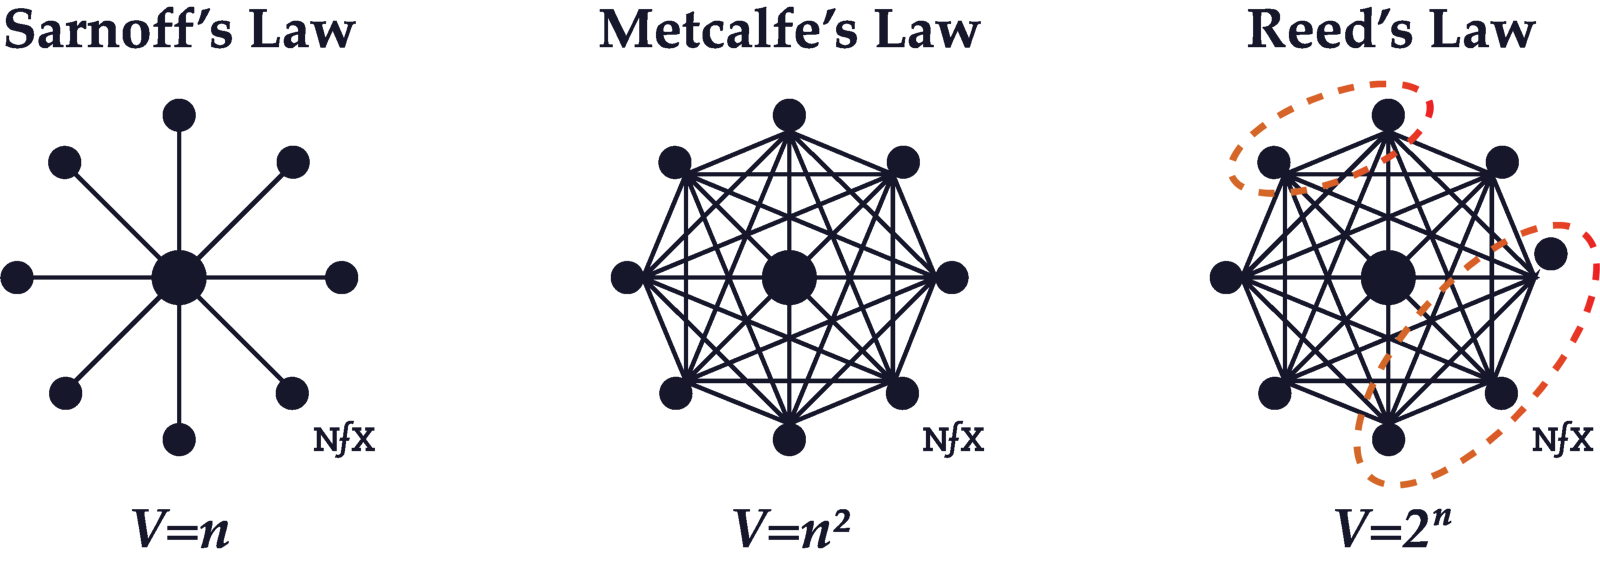
\includegraphics[width=0.85\textwidth]{./images/rsz_metcalfe.png} 
    \caption{Comparing Sarnoff's, Metcalfe's, and Reed's Laws \cite{metcalfs-law}}
\end{figure}

\noindent This above model demonstrates how connections within a telecommunications system increases the value of the system exponentially.
Combining this with constellation tokens and NXS, one is able to realize this exponential value through the ensuing strategies:

\begin{enumerate}
    \item \textbf{Economics:} Supply and demand drive token's valuation and cost per byte. [\ref{satellite-revenue}]
    \item \textbf{Technology:} Advancements such as unique services drive constellation's economic value. [\ref{additional-services}]
    \item \textbf{Expansion:} Revenue generated from an increase in your total amount of satellites realized by growth in the entire system. [\ref{no-monopolies}].
\end{enumerate}

\noindent This value is dispersed among constellation owners, enabling group control and decision making for each constellation as described in the following subsection.

\subsubsection{Tokenized Satellites}
\label{tokenized-satellites}

Tokenization systems can be applied to govern constellation ownership and therefore entitlements accordingly.
This ultimately provides individuals the opportunity to own part of the physical infrastructure of Nexus, while earning an ROI from the revenue the constellation produces.
The following describes the fundamental qualities of tokenized satellites:

\begin{enumerate}
    \item \textbf{Represented:} Each constellation is represented by a unique set of fungible tokens.
    \item \textbf{Ownership:} Ownership is maintained by equity in the quantity of fungible tokens.
    \item \textbf{Revenue:} Revenue generated from constellation is dispersed to token holders.
\end{enumerate}

\noindent As outlined above, the system acts as a technological mechanism for individuals to pool resources and deploy their own satellite cooperatives that will produce revenue in return.
This is fundamental to creating group oriented ownership systems, and abilities to share in the success in hardware deployments.
We believe this can be an equalizing force, by producing economic opportunity to individuals where it was not there previously.



\subsection{Incentives}

Incentives are an essential aspect of the open cryptographic system we have described in this paper. 
In the following subsections we will outline different techniques to provide both positive incentives and negative disincentives that will direct participants to creating as much cooperative value to the whole as possible, while simultaneously generating sufficient revenue that negates the desire to attempt gaming of the system.


\subsubsection{De-Monopolization}
\label{no-monopolies}

In order for the system to function well into the future, it must be able to resist the tendency for monopolies to form.
This is especially true when it comes to ISP's, as most people only have one ISP covering their area.
The NP must protect against this tendency, through consensus oriented mathematical weighting: \\

\begin{equation}
\resizebox{.33\hsize}{!}{$D_b = \mathlarger{\frac{1}{1 + 10\cdot e^{-x + 6}}}$ }
\end{equation}

\bigskip
\noindent Our mathematical model as a function of constellation and system sizes follows a sigmoid function.
This models $x$ as the constellation's relative size, achieved with ($x = \frac{t}{n}$) such that $n$ is the total satellites under single identity, and $t$ is the total registered satellites in the system.

\pagebreak
\begin{figure}[h]
    \centering
    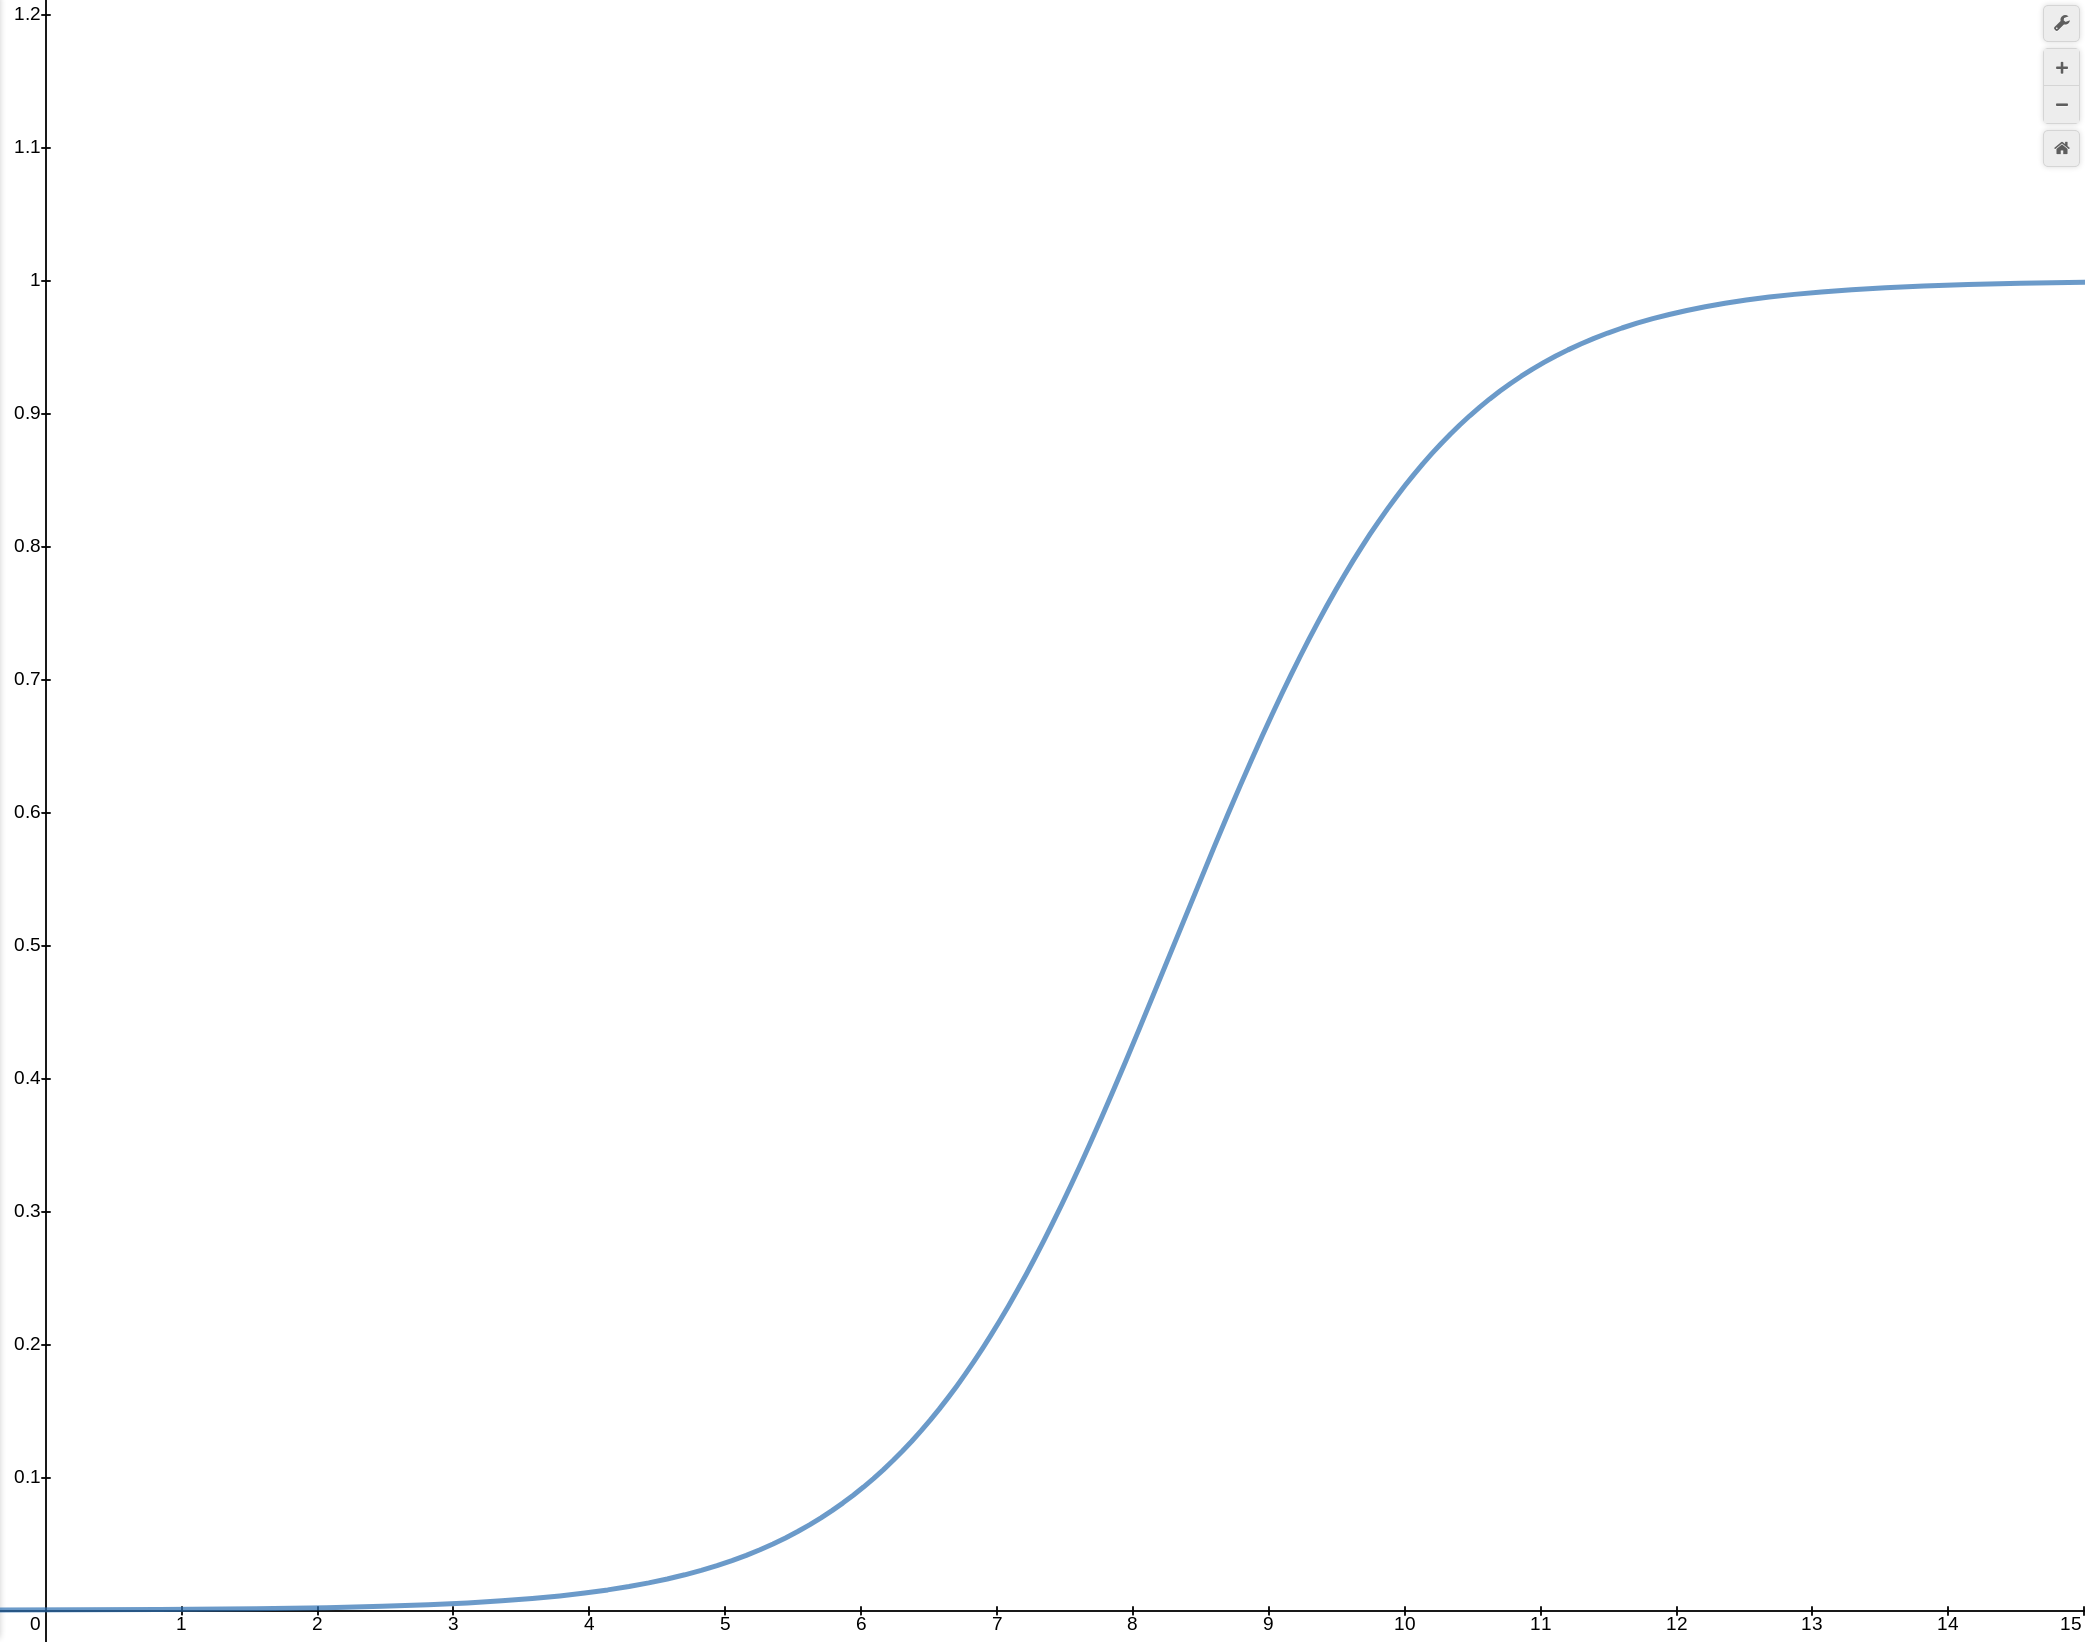
\includegraphics[width=0.8\textwidth]{./images/rsz_sigmoid.png}
    \caption{Relationship of selection bias ($y$) vs inverse of relative size ($x$)}
\end{figure}

\noindent Equation (7) begins decay of selection bias $\{0 \leq y \leq 1$ and $x \leq 12\}$, meaning as ownership exceeds $8.33\overline{3} \%$, constellation will begin receiving penalties in the form of idle hardware.

\begin{equation}
    \resizebox{.20\hsize}{!}{$S_b = D_b \cdot R$ }
\end{equation}

\bigskip
\noindent Equation (8) describes selection-bias ($S_b$) as a relationship between reputation ($R$) and de-monopolization boundary ($D_b$) demonstrating how $S_b$ is increased by increasing $n$ and $t$ proportionally to $\{\frac{t}{n} \leq 0.0833\overline{3}\}$ to maintain full reputation ($R$) in selection bias.
This has a direct relationship with revenue, as increasing $n$ proportional to $t$ yields a higher rate of return.


\subsubsection{Duplication Penalties}

\noindent This strategy encompasses making it less profitable to deploy multiple cooperatives that contain less satellites, as a means to bypass the above de-monopolizing tactics. 
In order to fulfill this requirement, we need to apply functions in a way that constellations that are rooted to single identities and larger number of satellites will over time generate more weight and therefore revenue than many identities with smaller number of satellites.

\begin{figure}[h]
    \centering
    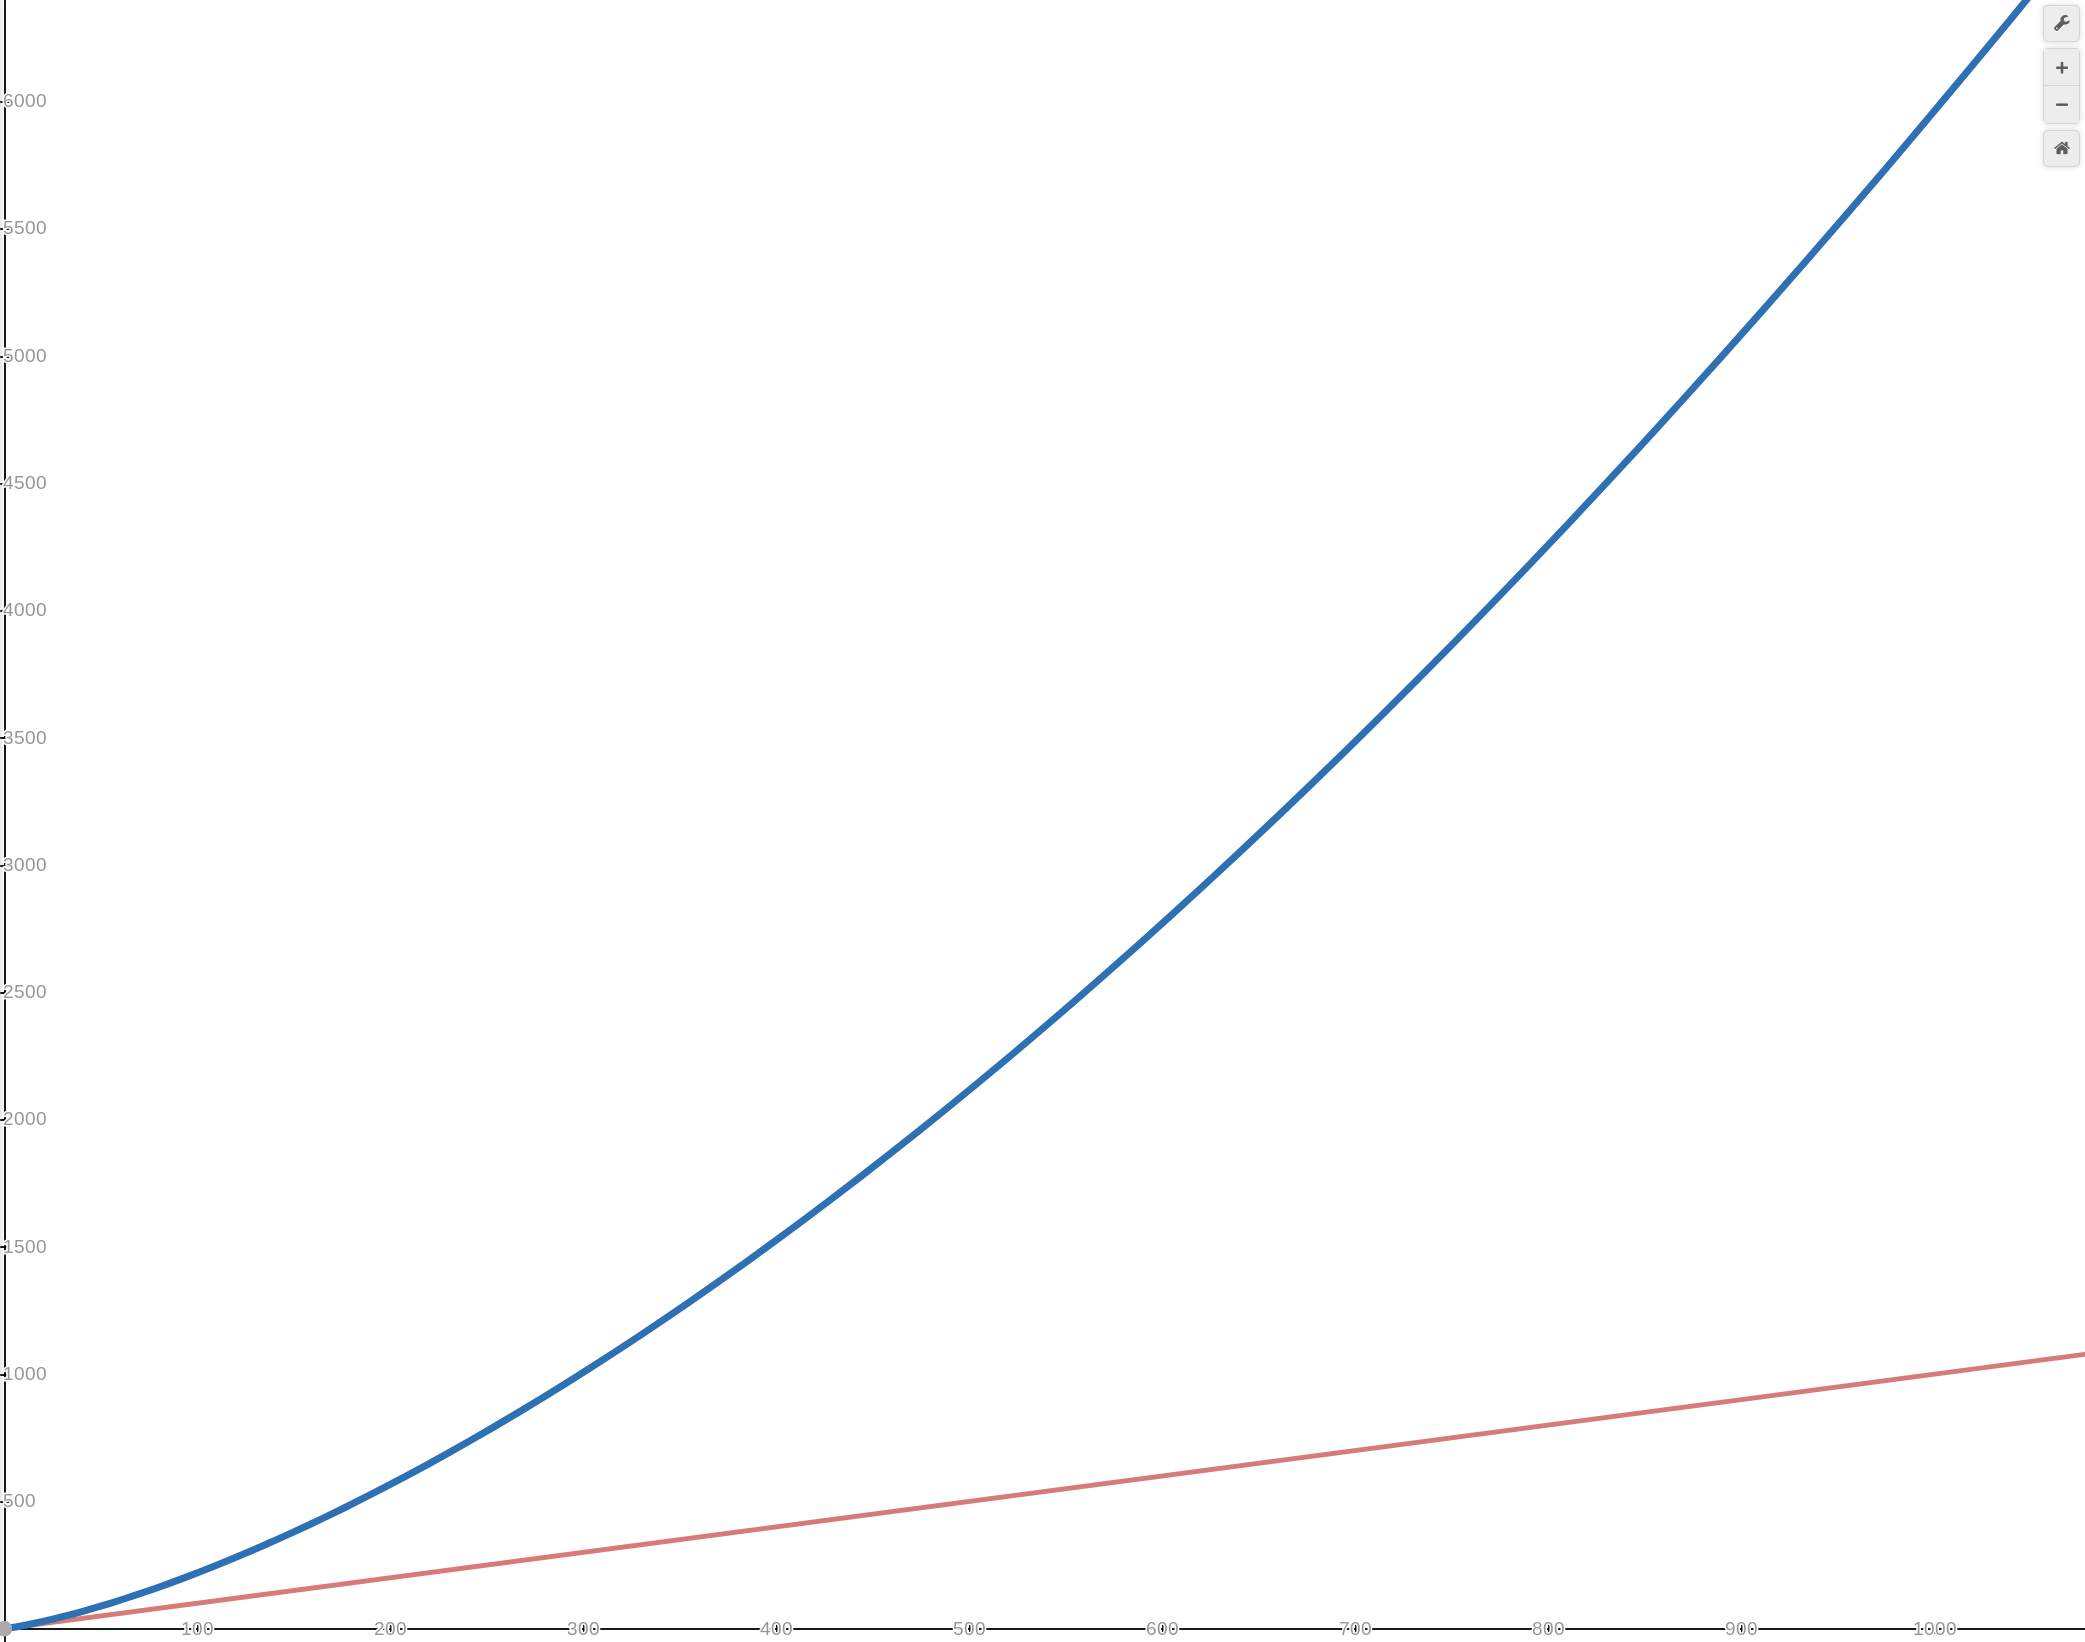
\includegraphics[width=0.80\textwidth]{./images/rsz_duplication.png}
    \caption{Growth in exponential weight (blue) vs duplicates (red)}
\end{figure}

\smallskip
\noindent We do this by producing a weighted bias of ($n^{\Phi}$) relative to individual constellation size, to produce higher economic value for consolidated constellations rather than many individuals.
The following equation models this relationship:

\begin{equation}
    \resizebox{.25\hsize}{!}{$W = \mathlarger{\frac{n^{1.618}}{14.4}} + n$ }
\end{equation}

\bigskip
\noindent The above equation describes our mathematical model that will make sybil attacks with new identities de-monetized and reduced in overall influence.
This will act as a direct disincentive by giving the system a common reference point to identify and thwart malicious actors from gaming the system.



\subsection{Reputation}

Reputation services are fundamental to maintaining open access standards, and ensuring the continued growth in the security of the system.
Reputation in our implementation and designs takes an important equalizing force and converts this into cryptographic proofs: time. 
The following Equation (10) and Equation (11) illustrate how the reputation is formulated:

\begin{equation}
    \resizebox{.2\hsize}{!}{$R = W \cdot T$ }
\end{equation}

\subsubsection{Hosting}

Reputation is part of what will fuel the selection bias as described in Equation (8).
This reputation will have a direct correlation with value produced in the system, as an inverse relationship between active contracts ($c_a$) and total contracts ($c_t$):

\begin{equation}
    \resizebox{.4\hsize}{!}{$T = \mathlarger{\sum}_{i=1}^{\infty} \frac{\min{(c_a, c_t)}}{c_t} \cdot i$ }
\end{equation}

\bigskip
\noindent In Equation (11) we see the total time ($T$) earned towards the reputation, modelled over the sum of intervals ($i$) designated as specific time-frames with snapshots of the active contracts ($c_a$) divided by total contracts ($c_t$) of the previous interval.
The result of this model, is the growth of the total time earned proportional to the percent of active contracts (\textit{min} ensures no inflated time rewards by enforcing $\{0 \leq c_a \leq c_t\}$ as the valid range), creating penalties for terminated contracts in that specific interval (i.e. a new interval begins by setting $c_a = c_t$, concluding with $\Delta c_a$ reflected at $i$).
This is then multiplied with one's weight ($W$) to derive the constellation's hosting reputation ($R$) and therefore selection bias ($S_b$) [\ref{no-monopolies}].


\subsubsection{Network}
\label{network-reputation}

Routing on the network will require that each ground station, satellite, and client to maintain a network reputation that reflects contributions to their geo-spacial location.
This allows cost of access to be determined by contributions to that local network, which protects against DDOS attacks, and bad actors leaching off the system while also allowing the basic access to the networks to be little to no cost.
This is imperative for safely connecting the many billions of people around the globe that are currently without the Internet.


\subsubsection{Maturation}

Part of the reputation system, is a phase we term the ``Maturation Period'' in which only a select few hard-coded satellite cooperatives can exist and inter-operate.
The requirement of this maturation period is to provide a window of time where the technology can be fully formed and moved to production ready implementations, while simultaneously providing security properties if the initial cooperatives are selected carefully.
After this period expires, through cryptographic consensus methods, the network will open up to new participants to join the routing and data selection system.
The de-monopolization techniques [\ref{no-monopolies}] require an initial data-set to measure against, which would not be possible without this maturation period.
We expect this maturation period to last a few years, after which hardware vendors can be ready for the new consumer demand for launches of new satellite cooperatives.


\subsubsection{Geo-Spacial Binding}

Since a large part of the security and game theory is ensured through the above mathematical models, we need to ensure that the count, or total number of active satellites is tallied accurately.
We are able to do this as a byproduct of our topologically independent routing system [\ref{software-routing}], that relies on locality and physical locations to operate.
Network Reputation [\ref{network-reputation}] provides this data-set for Geo-Spacial Binding (GSB), using relative positions to one another to compute and register new satellites in the system.
Coupled with ground station GSB and verification ensures that deployment of new cryptographic identities that represent physical hardware is not trivial to complete without the actual hardware (i.e. no hosting of many identities on a single satellite).




\section{Security Considerations}

In this section, we will describe the different security considerations that need to be taken into account to produce a well behaved telecommunication protocol.
We borrow techniques and attacks from our current technologies, in order to project the possible attacks upon the system and generate appropriate counter-measures.


\subsection{Common Vulnerabilities}

Commercial hardware products are rife with back-doors and fundamental flaws leaving even the most secure designs vulnerable to compromise.
Advancements in manufacturing and innovative designs are allowing even nanotechnology scale semiconductor structures to be packed with increasing density to boost computational capacity. 

\bigskip
{\large\noindent\textbf{Common attacks include \cite{HW-attacks}:}}

\begin{enumerate}
\item \textbf{Backdoors:} Manufactured for remote support, diagnostics, malware or other penetrative purposes; the presence of hidden methods for bypassing normal computer authentication systems.
\item \textbf{Eavesdropping:} By gaining access to protected memory without opening other hardware.
\item \textbf{Interruption:} Inducing faults, causing the interruption of normal behavior.
\item \textbf{Tampering:} Hardware modification tampering with invasive operations; hardware or jailbroken software.
\item \textbf{Counterfeiting:} Product assets that can produce extraordinary operations, and those made to gain malicious access to systems.
\end{enumerate}

\noindent We aim to overcome at least some of these deficiencies with LX-OS, primarily targeting IoT and Micro-Satellites for our first iteration.

\subsection{Privacy Leakage}
\label{privacy-leakage}

Mapping entries need to account for privacy related requirements, as using a GSL system can reveal personally identifying information that could compromise an individual's GSL and therefore physical safety. 
We resolve this deficiency through the following methods:

\begin{enumerate}
    \item \textbf{Aggregation:} Using aggregated mapping, only ground stations of that local WRL contains the GSL's.
    \item \textbf{Proxies:} More novel techniques where the GSL themselves are not registered but rather a proxy registers their own GSL into the local WRL instead of the user.
    \item \textbf{Locality:} Precise GSL's can only be stored by physically local nodes as they will already know each other's true physical locators.
\end{enumerate}



\subsection{GPS Vulnerabilities}

GPS systems are susceptible to several types of interference and manipulation. 
Coordinates can be jammed, spoofed or interrupted by environmental conditions easily. 
These are a few of the security considerations to take into account related to our stateless GSL routing system. 
In the following subsections we will describe this attack surface, and identify key qualities that will be needed to ensure a stable operating of the networks even under heavy attack.

\begin{figure}[h]
    \centering
    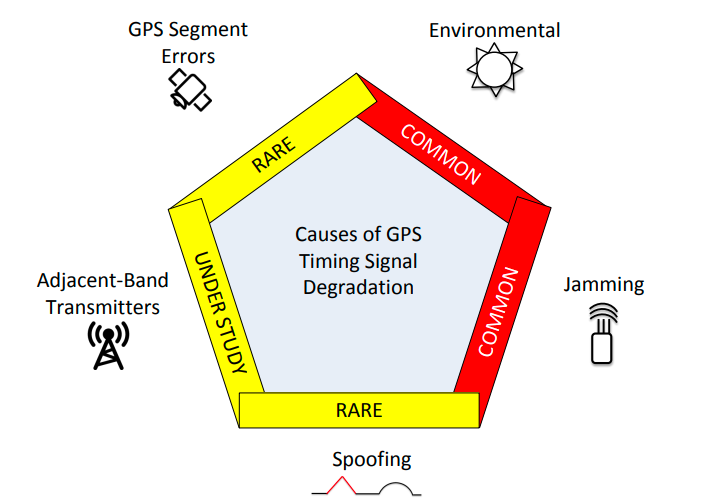
\includegraphics[width=0.7\textwidth]{./images/rsz_gps_signal.png}
    \caption{Causes of GPS Signal Degradation \cite{GPS-vulns}}
\end{figure}


\subsubsection{Spoofing}

GPS Spoofing is a well known technique, and has the potential to cause only minimal problems for the individual that attempts it.
However, there is potential for positioning, navigation and timing spoofing that can affect a broad array of services and devices \cite{GPS-signal}.
Essentially, with the system relying on GPS coordinates for the GSL routing system, one spoofing their GPS coordinates will result in themselves being locked from the network, as they will not be able to receive packets at their given GSL.


\subsubsection{Interference}

Signal jamming and manipulation is large  part of the attack surface of the GPS oriented routing system.
Environmental conditions can be artificially influenced to induce desired disruptions or derived from natural causes.
These could all cause artificial results or packet loss to a node attempting to connect.
The following graphic provides and overview of the GPS radio signal production.

\begin{figure}[h]
    \centering
    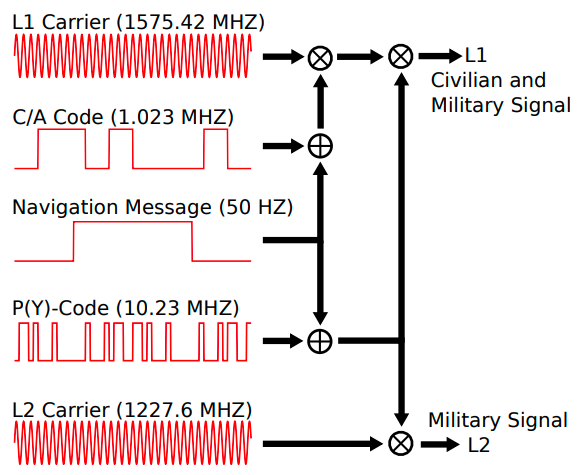
\includegraphics[width=0.7\textwidth]{./images/rsz_gps_types.png}
    \caption{GPS Signal Production Types \cite{GPS-signal}}
\end{figure}

\noindent We overcome these threats by applying industry leading best practices, redundancy checking, and high directional gain, making it difficult to manipulate multiple beams from any single location.



\subsection{DDoS Attacks}

Distributed Denial of Service (DDoS) Attacks are powerful weapons for adversaries that wish to censor and destroy communication channels between peers. 

\begin{figure}[h]
    \centering
    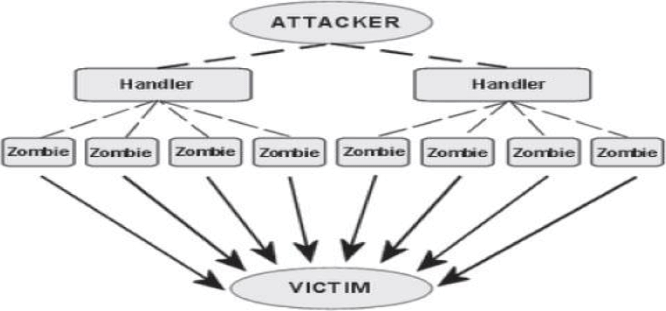
\includegraphics[width=0.5\textwidth]{./images/rsz_ddos_arch.png}
    \vspace{-10pt}
    \caption{Architecture of a DDOS Attack \cite{DDoS-arch}}
\end{figure}

\pagebreak
\noindent In the next subsections we outline the attack surface of DDoS threats on our software defined routing designs, and demonstrate how these strategies will become increasingly ineffective for denying clients access to key services.


\subsubsection{DDoS Against Routers}

In this subsection we describe DDoS attacks on routers and how this is one of the primary concerns and nearly unsolvable issues on the Internet, as pipes do not generally have physical layer protection and rely on limited hardware capabilities for routers or third party services.

\begin{enumerate}
    \item \textbf{Hardware:} Hardware based routers have limited computing cycles available.
    \item \textbf{Latency:} They are prone to being overpowered by DDoS traffic and not being able to drop packets fast enough.
    \item \textbf{Reputation:} Reputation throttles packet throughput, and physical circuit breakers through steering of phased array antennas make DDoS attacks against the software defined routers very difficult to achieve.
    \item \textbf{Computing:} Software defined routing affords the routing software more computing cycles and faster clocks in the case that a physical circuit breaker is not needed.
\end{enumerate}

\noindent Software Defined Routers provide us many opportunities to protect the routing system against abuse, in ways that were not previously possible.


\subsubsection{Physical Layer Protection}

A pipe, or physical cable transmitting data along in the Internet generally cannot be physically disconnected for protection. 
The result of this, when DDoS incidents occur, is the static routers cannot drop packets fast enough and can become overpowered in data centers, and even entire ISP's.
This limitation of hardware defined routing, and the architecture of the Internet reliance on material mediums, prevents physical layer protections.

\pagebreak
\begin{figure}[h]
    \centering
    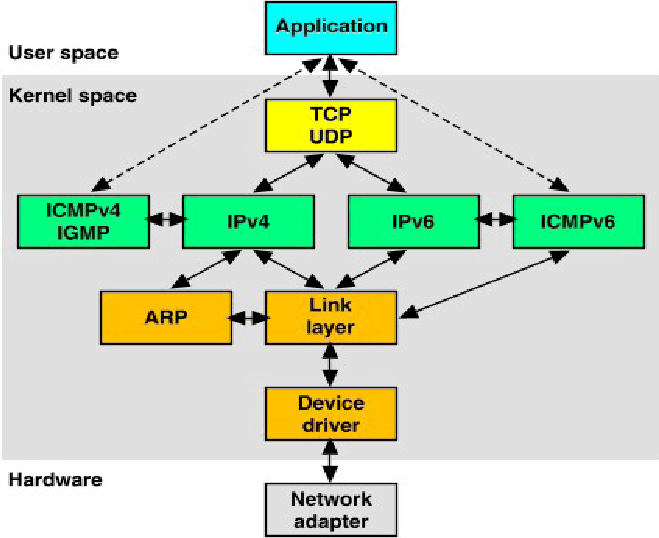
\includegraphics[width=0.6\textwidth]{./images/rsz_packet_flow.png}
    \caption{Packet Flow for OSI Reference Model \cite{Packet-flow}}
\end{figure}

\noindent Using phased array antennas, one can determine link duration from packet flow vs reputation cutting the link by pointing to a different direction that protects the overall routing system on the physical layer.
This reduces the attack surface to local RF saturation limitations, where an actor would be restricted to saturating the airwaves as a localized Denial of Service exploit.


\subsection{Packet Sniffing}
\label{packet-sniffing}

Phased array antennas protect against packet sniffing requiring bad actors to be in direct line of sight to compromise network traffic.  
This has been widely verified \cite{Beamform-sec} with recent advancements that are improving capabilities. 
The following depiction reflects a user (Bob) isolated by beam-forming in the enclosed exposure region.

\begin{figure}[h]
    \centering
    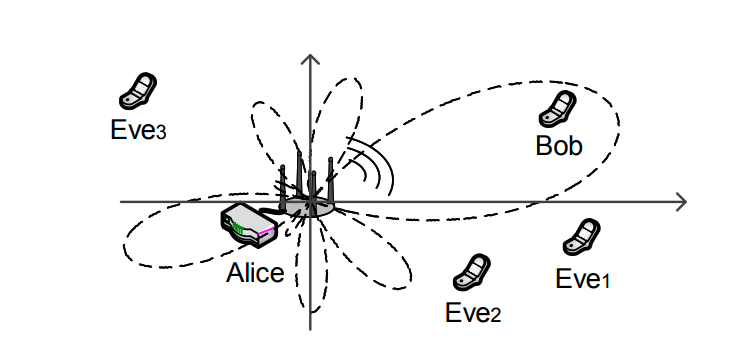
\includegraphics[width=0.65\textwidth]{./images/rsz_beamform_isolation.png}
    \caption{Beam-forming Isolation from Exposure Diagram \cite{Beamform-ER}}
\end{figure}

\noindent The following list describes the security precautions planned to reduce the attack surface of packet sniffing related exploits:

\begin{enumerate}
    \item \textbf{Beam-forming:} Phased Array antennas create noise perpendicular from beam-forming requiring attacker to point directly in the line of sight.
    \item \textbf{Directional:} Using high gains (33 dBi), the signals will have high directional gain, making packet sniffing increasingly difficult on the physical layer.
    \item \textbf{Encryption:} Combined with encryption techniques given line of sight was gained to jam or sniff a beam, the packets themselves would be of no value to an attacker.
\end{enumerate}

\noindent We anticipate the widespread use of these antenna systems can produce overall more secure communication networks with less potential for abuse from bad actors.

\subsubsection{Man in the Middle}

Man in the Middle (MitM) attacks involve intercepting or altering communications between peers or systems to achieve an objective. The next diagram depicts a MitM attack on a Key Exchange (KE) protocol.

\begin{figure}[h]
    \centering
    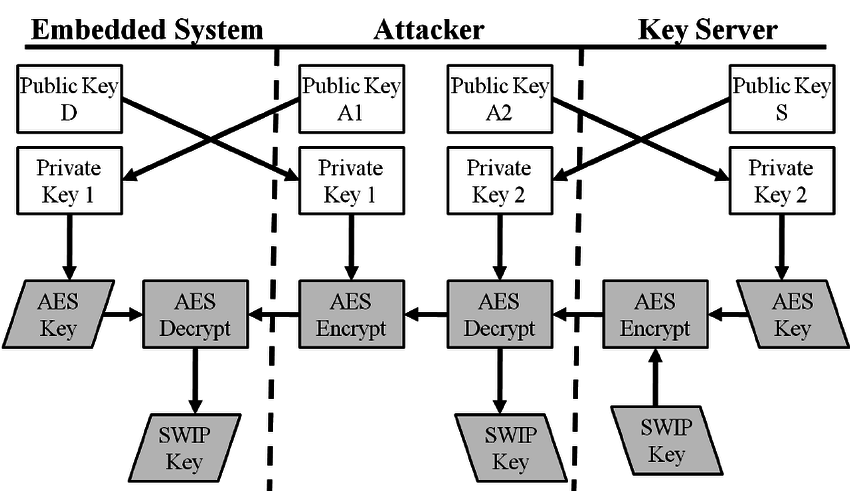
\includegraphics[width=0.7\textwidth]{./images/rsz_mitm.png}
    \caption{MitM Attacks on Key Exchange Protocols \cite{MitM-attack}}
\end{figure}

\begin{center}
     
\end{center}

\noindent Using the concepts described in the previous sections, newly augmented into the system, we can greatly reduce the capabilities and effectiveness of MitM attacks.
The following describes how we achieve this:

\begin{enumerate}
    \item \textbf{Authenticate:} Protect against MitM attacks through the use of distributed and trust-less authentication techniques.
    \item \textbf{Root of Trust:} Certificates for Transport Layer Security (TLS) communication shall be verified from blockchain entries, that also contain the above mentioned authentication data.
\end{enumerate}

\noindent At the time of writing, TLS 1.3 \cite{TLS1.3} is the most current version that resolves a number of critical security, privacy and performance problems. 

\subsubsection{Cache Poisoning}

ARP caches can be poisoned by an attacker on your network, so candidates such as S-ARP can be implemented as a protection mechanism.
The following list describes further options for protecting critical mappings:

\begin{enumerate}
    \item \textbf{Authenticate:} For all cell communication, everything must be authenticated for security dependent mappings i.e. MAC $\longmapsto$ IP (ARP), EID $\longmapsto$ RLOC (LISP), etc.
    \item \textbf{Encryption:} TLS 1.3 communication must be enabled by default to ensure no plain-text packets are available, it must become a fundamental standard.
\end{enumerate}

\noindent All certificates will adhere to updated release specifications at minimum as they are made available. 
Additionally, advanced blockchain security functionality is planned to reinforce this key infrastructure.

\subsection{Post Quantum Security}

In preparation of a Post Quantum (PQ) age, we intend to remain constantly vigilant and use cryptographic standards that assure resistance to PQ related security exploits.
The below list outlines our PQ security requirements, to satisfy our Digital Signature Algorithm (DSA) and Key Exchange (KE) mechanisms:

\begin{enumerate}
    \item \textbf{SABER:} We will use PQ encryption techniques such as SABER \cite{SABER} to ensure PQ-KE channels over both IP/NP
    \item \textbf{FALCON:} Digital signatures need to be verified and generated using PQ techniques. We use lattice based DSA's, namely FALCON \cite{FALCON} for verification of identities and reputation.
\end{enumerate}

\section{Conclusion}

In this paper we have outlined the core architecture necessary for a novel communication protocol to be realized, and defined new qualities that can be facilitated and nurtured by open connection.
We believe that at such a crucial time for humanity, it is becoming more apparent that we need to be looking at our current challenges with new perspectives.
Our societies needs new technologies that are designed to serve the people, to benefit them directly and give them ownership in the overall infrastructure.
With ISM Frequencies, Affordable Hardware, Phased Array Antennas, Economic Models, GSL Routing, LISP Mapping, and WRL Blooms we have now demonstrated that this is not only just feasible, it is well within reach.
When fully achieved, this architecture and methodology can open the world to the stars, re-awakening their imaginations, and generating opportunities where none existed before.
A \textit{true} currency powering a \textit{true} Internet, Nexus will guide these emerging economies into a cycle of new fortuity, giving us the chance to prove what is now possible.


\bigskip 
\begin{center}
\textbf{ad astra credo}
\end{center}



\pagebreak
{\noindent\Large\textbf{List of Contributors}}
\bigskip

\noindent The following list contains contact information for each contributor, listed in alphabetical order.

\begingroup
\parindent 0pt
\parskip  0pt

\begin{enumerate}

\item
\printcontributor{BA}

\item
\printcontributor{April}

\item 
\printcontributor{Cantrell}

\item
\printcontributor{Hauk}

\item
\printcontributor{Shea}

\item 
\printcontributor{Victor}

\end{enumerate}

\endgroup


\pagebreak
\begin{thebibliography}{7}


\bibitem{Internet-History}
A Brief History of the Internet \& Related Networks
\url{https://www.internetsociety.org/internet/history-internet/brief-history-internet-related-networks}

\bibitem{ARPANET}
ARPANET
\url{https://en.wikipedia.org/wiki/ARPANET}

\bibitem{NetworkOSI}
The OSI Reference Model and Protocols
\url{https://flylib.com/books/en/2.567.1.38/1/}

\bibitem{Phased-Arrays}
Phased Array Antennas for Satellite Applications
\url{https://rftonics.ksu.edu.sa/node/1176}

\bibitem{ISM_Table}
ISM Frequencies
\url{https://en.wikipedia.org/wiki/ISM_band}

\bibitem{RF-Exposure}
Radiofrequency and Microwave Radiation
\url{https://www.osha.gov/radiofrequency-and-microwave-radiation/health-effects}

\bibitem{karman-line}
What Is The Karman Line?
\url{https://www.worldatlas.com/articles/what-is-the-karman-line.html}

\bibitem{ISM_Limits}
Electronic Code of Federal Regulations
\url{https://www.ecfr.gov/cgi-bin/text-idx?SID=eed706a2c49fd9271106c3228b0615f3&mc=true&node=pt47.1.15&rgn=div5#se47.1.15_1247}

\bibitem{data-rates}
AP510 Series Access Point Datasheet
\url{https://www.arubanetworks.com/assets/ds/DS_AP510Series.pdf}

\bibitem{MCS-Table}
802.11ax MCS Rates Table
\url{https://www.rfwireless-world.com/Terminology/802.11ax-MCS-Rates-Table.html}

\bibitem{starlink}
LEO satellite networks
\url{https://leosatsim.github.io/}

\bibitem{bloom-filters}
Bloom Filters - Introduction and Implementation
\url{https://www.geeksforgeeks.org/bloom-filters-introduction-and-python-implementation/}

\bibitem{CDN-usage}
 Data volume of global content delivery network internet traffic from 2017 to 2022 
\url{https://www.statista.com/statistics/267184/content-delivery-network-internet-traffic-worldwide/}

\bibitem{LISP}
The Locator/ID Seperation Protocol 
\url{https://tools.ietf.org/html/rfc6830}

\bibitem{uberlay}
Uberlay Interconnection of Multiple LISP Overlays
\url{https://tools.ietf.org/html/draft-moreno-lisp-uberlay-02}

\bibitem{S-ARP}
S-ARP: a Secure Address Resolution Protocol
\url{https://www.acsac.org/2003/papers/111.pdf}

\bibitem{kernel-architecture}
Comparison between Monolithic and Microkernels
\url{https://www.researchgate.net/figure/Comparison-between-a-monolithic-kernel-design-A-and-a-microkernel-B_fig1_274076584}

\bibitem{seL4}
The seL4 Microkernel
\url{https://sel4.systems/}

\bibitem{buffer-overflow}
Buffer Overflow Expoit, Part 3
\url{https://priyasloka.wordpress.com/2018/04/13/buffer-overflow-exploit-part-3/}

\bibitem{seL4-syscall}
Verified Protection Model of the seL4
Microkernel
\url{https://www.researchgate.net/publication/221160526_Verified_Protection_Model_of_the_seL4_Microkernel}

\bibitem{merkle-tree}
Merkle Trees
\url{https://brilliant.org/wiki/merkle-tree/}

\bibitem{metcalfs-law}
The Network Effects Bible
\url{https://medium.com/@nfx/the-network-effects-bible-c6a06b8ae75b}

\bibitem{HW-attacks}
Hardware attacks, backdoors and electronic component qualification
\url{https://resources.infosecinstitute.com/topic/hardware-attacks-backdoors-and-electronic-component-qualification/}

\bibitem{GPS-vulns}
ATIS GPS Vulnerability Report
\url{https://www.gps.gov/governance/advisory/meetings/2016-12/calabro.pdf}

\bibitem{GPS-signal}
CMU Study: GPS Software Attacks
\url{https://users.ece.cmu.edu/~dbrumley/pdf/Nighswander\%20et\%20al._2012_GPS\%20software\%20attacks.pdf}

\bibitem{DDoS-arch}
Twords the use of BPANN Technique for Mitigating Layer 4 DDoS Attack in Electronic Voting
\url{https://www.researchgate.net/publication/329102112_TOWARDS_THE_USE_OF_BPANN_TECHNIQUE_FOR_MITIGATING_LAYER_4_DDOS_ATTACK_IN_ELECTRONIC_VOTING}

\bibitem{Packet-flow}
Network Traffic Analysis and Intrusion Detection Using Packet Sniffer
\url{https://www.researchgate.net/publication/232625696_Network_Traffic_Analysis_and_Intrusion_Detection_Using_Packet_Sniffer}

\bibitem{Beamform-sec}
Creating secure wireless regions using configurable beamforming
\url{https://core.ac.uk/download/pdf/33581035.pdf}

\bibitem{Beamform-ER}
Security Optimization of Exposure Region-based Beamforming with a Uniform Circular Array
\url{https://pureadmin.qub.ac.uk/ws/files/137758457/TCOM_Final_Manuscript.pdf}

\bibitem{MitM-attack}
Securing Software Intellectual Property on Commodity and Legacy Embedded Systems
\url{https://www.researchgate.net/publication/242668335_Securing_Software_Intellectual_Property_on_Commodity_and_Legacy_Embedded_Systems}

\bibitem{TLS1.3}
The Transport Layer Security (TLS) Protocol Version 1.3
\url{https://tools.ietf.org/html/rfc8446}

\bibitem{SABER}
SABER: IND-CCA2 secure Key Encapsulation Mechanism (KEM)
\url{https://www.esat.kuleuven.be/cosic/pqcrypto/saber/index.html}

\bibitem{FALCON}
FALCON: Fast Fourier LAttice-based Compact Signatures over NTRU
\url{https://falcon-sign.info/}



\end{thebibliography}

\end{document}